\section{Incident Analysis}
\label{sec:incident_analysis}

This section presents the empirical application of the B-SAFE framework to real-world security incidents. We analyze critical risk categories for each layer of the blockchain architecture, providing a formal specification, defense mechanism analysis, and risk prioritization based on our corpus of 647 incident entries (2016--2025).

\begin{figure}[H]
\centering
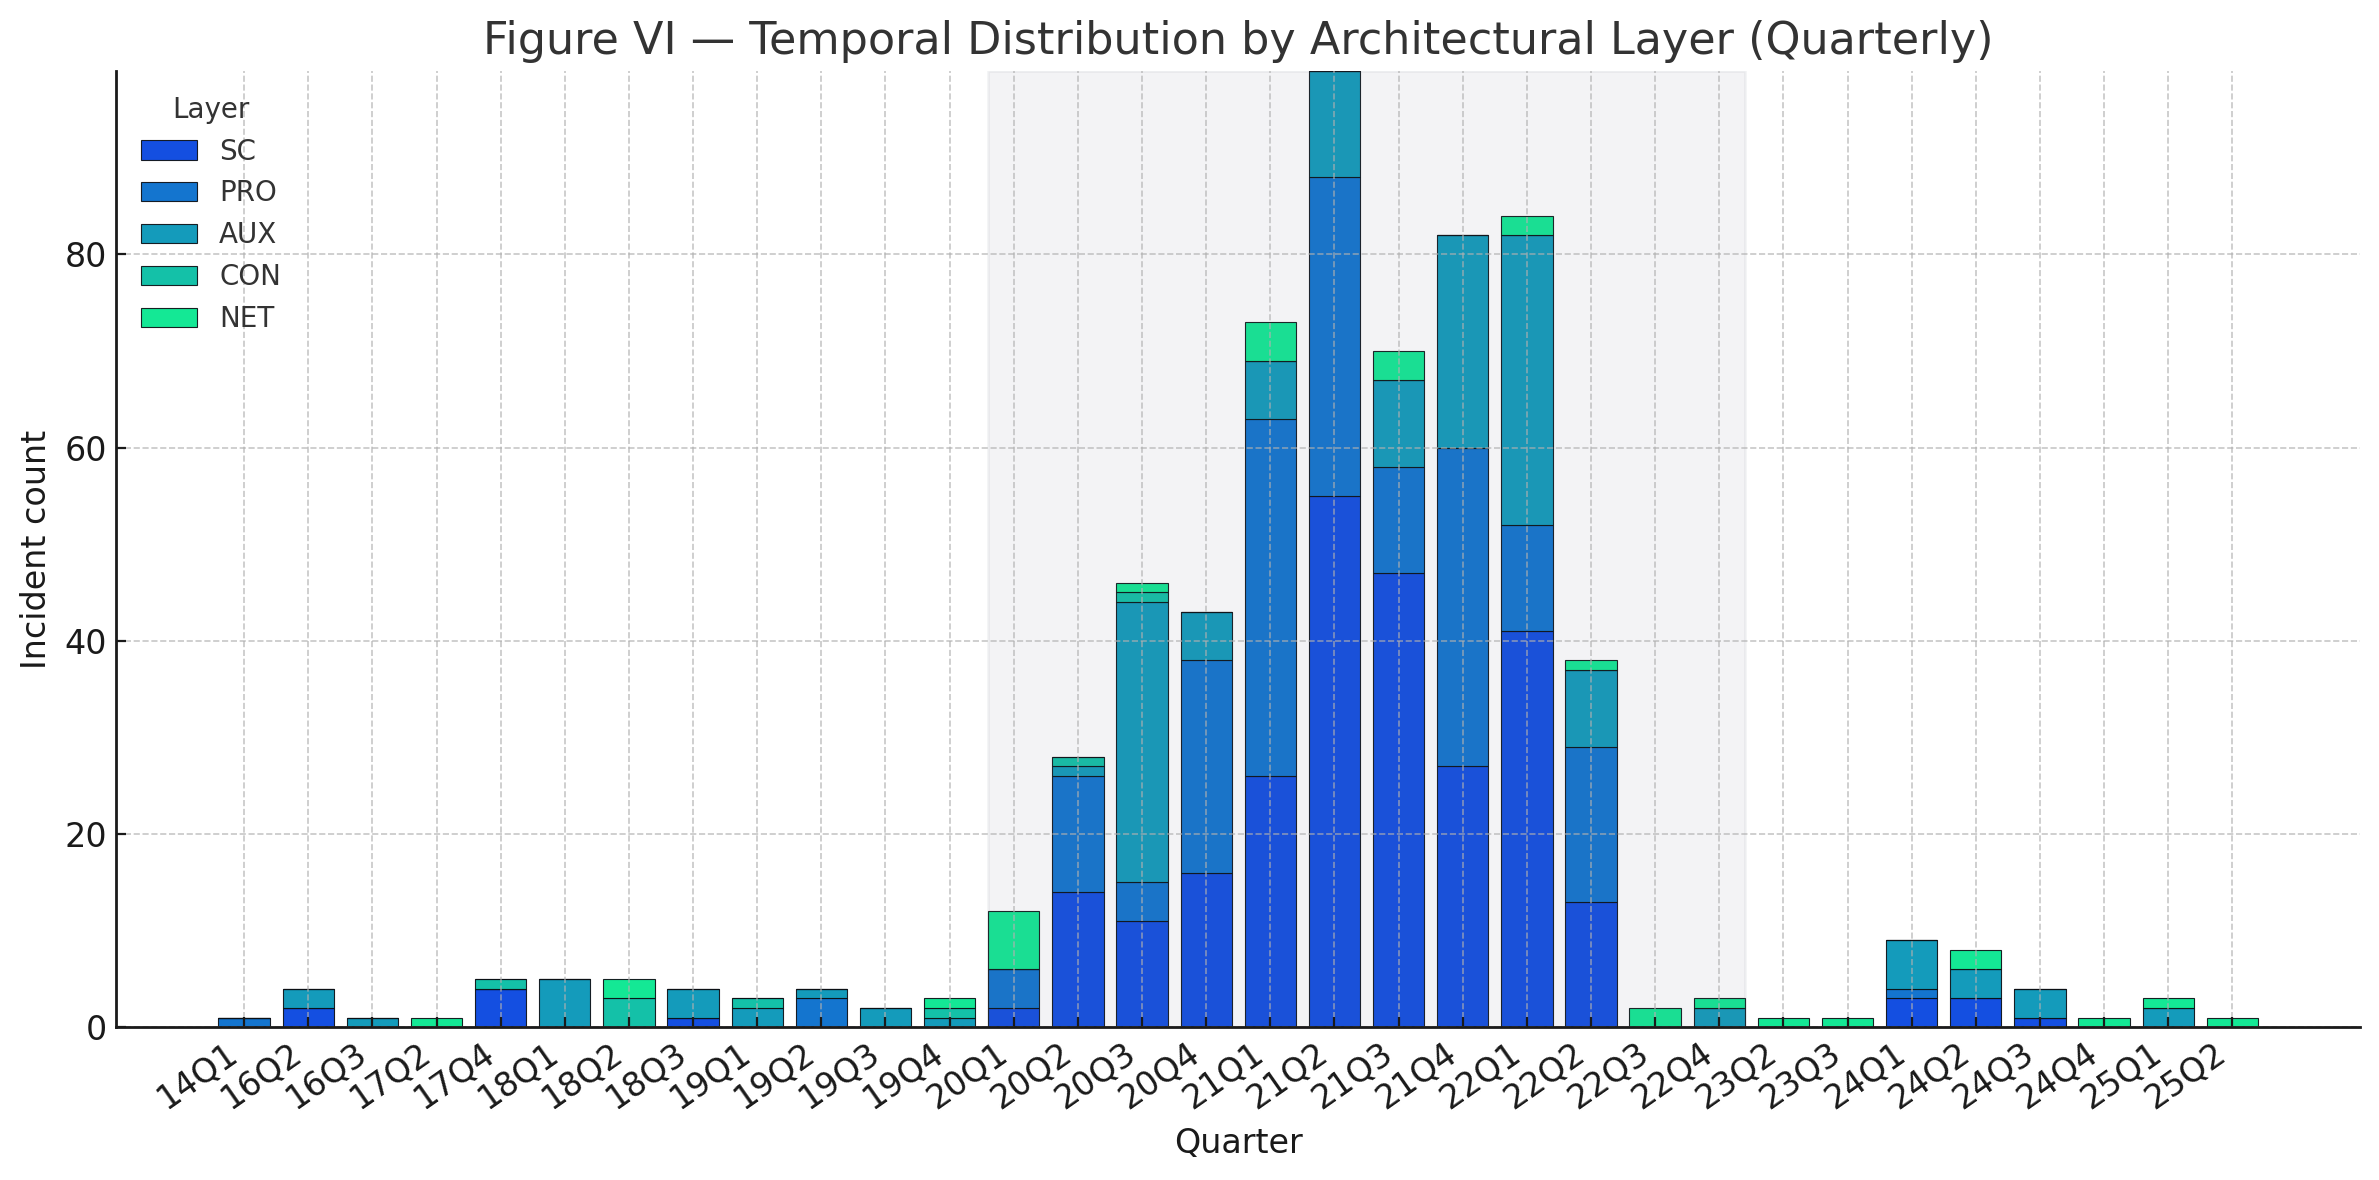
\includegraphics[width=0.4\textwidth]{../figure/fig6.png}
\caption{Temporal distribution of blockchain security incidents by architectural layer. Smart contract vulnerabilities consistently dominate, while DeFi protocol attacks surged during the 2020-2022 DeFi boom. Network and consensus layer incidents remain relatively rare but potentially catastrophic.}
\label{fig:incident_timeline}
\end{figure}

\begin{figure}[H]
\centering
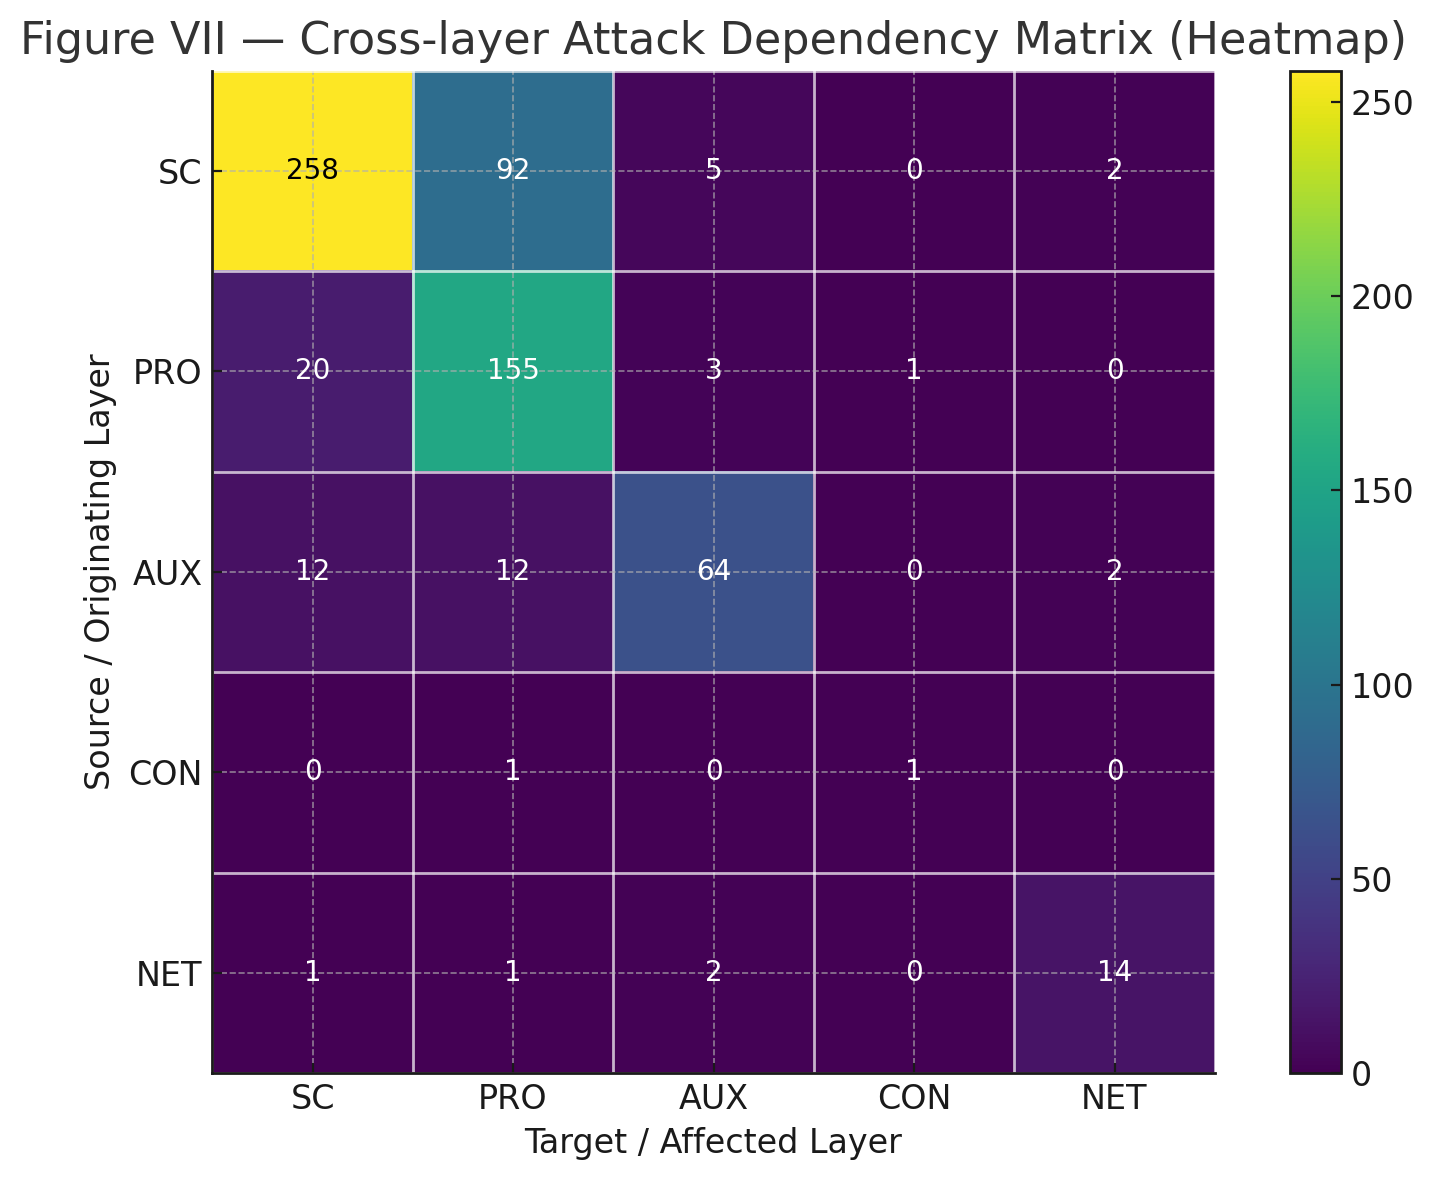
\includegraphics[width=0.4\textwidth]{../figure/fig7.png}
\caption{Cross-layer attack dependency matrix showing how vulnerabilities in one layer enable or amplify threats in others. Smart contract vulnerabilities frequently cascade to protocol layer issues, while protocol attacks often affect auxiliary infrastructure.}
\label{fig:cross_layer_dependencies}
\end{figure}

\subsection{Security Analysis of Consensus and Network Layers}
\label{sec:results_consensus_network}

\paragraph{Executive Summary}
Consensus-layer threats (e.g., majority attacks, selfish mining, PoS long-range) and network-layer threats (e.g., eclipse) undermine finality, ledger integrity, and reward fairness. Incidents cluster on minority chains or poorly peered networks, with cascading impact to exchanges and custodians. Enterprise controls map to: chain selection policies, value-sensitive confirmation thresholds, hashrate/validator concentration monitoring, peer-discovery hardening, trusted checkpoints (PoS), and SOC playbooks for reorg response.

\subsubsection{Risk Category CON-1: 51\% Majority Attack}

\paragraph{Formal Risk Specification}

\begin{itemize}
    \item \textbf{Preconditions (P):}
    \begin{itemize}
        \item \textbf{P1: Hash Rate Concentration:} An attacker or coalition acquires control over 50\% of the network's total mining hashrate \cite{Wang2019, Eyal2014}.
        \item \textbf{P2: Economic Viability:} The cost of acquiring the necessary hashrate, often rented from public markets like NiceHash, is lower than the potential financial gain from executing the attack \cite{Casino2019}. This is particularly true for smaller-cap blockchains.
    \end{itemize}

    \item \textbf{Threatened System Invariants (I):}
    \begin{itemize}
        \item \textbf{INV-1 (Ledger Immutability):} The core guarantee that past transactions are permanent is violated, as the attacker can forcibly rewrite the ledger's history \cite{Wang2019}.
        \item \textbf{INV-2 (Value Conservation):} The attacker can reverse their own transactions after they have been confirmed, leading to successful double-spends and the creation of fraudulent value \cite{Eyal2014}.
    \end{itemize}

    \item \textbf{Canonical Attack Sequence (S):}
    \begin{enumerate}
        \item \textbf{Preparation Phase:} The attacker sends cryptocurrency to a third party (e.g., an exchange) on the public chain \cite{Casino2019}.
        \item \textbf{Private Mining Phase:} Simultaneously, the attacker uses their majority hashrate to secretly mine an alternate, private version of the blockchain where the initial transaction never occurred \cite{Eyal2014}.
        \item \textbf{Reorganization Phase:} After the public transaction is confirmed and the attacker has withdrawn the exchanged assets, they release their longer private chain to the network. Following the "longest chain" rule, the rest of the network discards the original public chain and adopts the attacker's version \cite{Wang2019}.
        \item \textbf{Exploitation Phase:} The attacker's initial transaction is erased, yet they retain the assets from the exchange, completing the double-spend \cite{Casino2019}.
    \end{enumerate}
\end{itemize}

\paragraph{Enterprise Checklist Mapping}
\begin{itemize}
    \item \textbf{Architecture/Platform}: Avoid minority PoW chains for critical value; require PoS weak subjectivity checkpoints.
    \item \textbf{Operations}: Exchange confirmation policies calibrated to chain economic security; reorg runbooks.
    \item \textbf{Security}: Hashrate/validator distribution monitoring; hardened peer discovery; trusted node anchoring.
\end{itemize}

\paragraph{Defense Mechanism Analysis}

\begin{itemize}
    \item \textbf{Prevention Controls:}
    \begin{itemize}
        \item \textbf{C1.1 (Economic Security):}
            \begin{itemize}
                \item \textit{Mechanism:} Grow the network's total hash rate to a level where acquiring 51\% becomes prohibitively expensive \cite{Wang2019}.
                \item \textit{Trade-offs:} This defense is an emergent property of a chain's value and community size, making it difficult to "engineer" directly, especially for minority chains \cite{Eyal2014}.
            \end{itemize}
    \end{itemize}
    \item \textbf{Mitigation Controls:}
    \begin{itemize}
        \item \textbf{C2.1 (Increased Confirmation Requirements):}
            \begin{itemize}
                \item \textit{Mechanism:} Services, particularly exchanges, can wait for a much larger number of blocks to be mined on top of a deposit before crediting it \cite{Casino2019}. This forces an attacker to maintain the costly majority hashrate for a longer period.
                \item \textit{Trade-offs:} Significantly increases transaction settlement times and reduces usability \cite{Casino2019}.
            \end{itemize}
    \end{itemize}
    \item \textbf{Detection Controls:}
    \begin{itemize}
        \item \textbf{C3.1 (Hashrate Distribution Monitoring):}
            \begin{itemize}
                \item \textit{Mechanism:} Monitor the distribution of hashrate on public markets and be alerted to large, sudden accumulations of mining power pointed at specific chains \cite{Wang2019}. A successful reorganization is immediately detectable after the fact.
            \end{itemize}
    \end{itemize}
\end{itemize}

\paragraph{Empirical Incident Analysis}

\begin{itemize}
    \item \textbf{Case Study CON-1.1: Attacks on Ethereum Classic (ETC) and Bitcoin Gold (BTG)}
    \begin{itemize}
        \item \textbf{Incident Classification:}
            \begin{itemize}
                \item \textit{Precondition Analysis:} P1 and P2 were met as these are minority chains, and the necessary hashrate was readily and cheaply available for rent on public markets like NiceHash \cite{Casino2019, Eyal2014}.
                \item \textit{Invariant Violations:} Both INV-1 and INV-2 were catastrophically violated, allowing attackers to rewrite chain history and execute double-spends against exchanges, leading to tens of millions of dollars in fraudulent transactions \cite{Casino2019}.
                \item \textit{Defense Failures:} The targeted exchanges had insufficient C2.1 confirmation thresholds, underestimating the practical risk posed by the commodification of hashrate \cite{Eyal2014}.
            \end{itemize}
        \item \textbf{Quantitative Impact Assessment:}
            \begin{itemize}
                \item \textit{Direct Losses:} Tens of millions of dollars in fraudulent transactions across multiple incidents \cite{Casino2019}.
                \item \textit{Systemic Effects:} The events severely eroded trust in the security of smaller Proof-of-Work chains, leading to market cap decline and delistings from major exchanges \cite{Casino2019, Wang2019}.
            \end{itemize}
        \item \textbf{Counterfactual Analysis:}
            \begin{itemize}
                \item \textit{Prevention:} Had the exchanges implemented drastically higher C2.1 confirmation requirements tailored to the specific economic security level of these chains, the cost and duration of the attack would have likely become unprofitable, deterring the attacker \cite{Eyal2014}.
            \end{itemize}
    \end{itemize}
\end{itemize}

\subsubsection{Risk Category CON-2: Selfish Mining}

\paragraph{Formal Risk Specification}

\begin{itemize}
    \item \textbf{Preconditions (P):}
    \begin{itemize}
        \item \textbf{P1: Significant Hashrate Control:} An attacker, typically a large mining pool, controls a significant, though not necessarily majority, portion of the hashrate (e.g., >25\%) \cite{Eyal2014}.
        \item \textbf{P2: Network Latency Exploitation:} The attack relies on the unavoidable latencies of a global P2P network, which give the attacker a time advantage when strategically releasing their hidden blocks \cite{Eyal2014, Wang2019}.
    \end{itemize}

    \item \textbf{Threatened System Invariants (I):}
    \begin{itemize}
        \item \textbf{INV-3 (Fair Reward Distribution):} The invariant that a miner's expected rewards are proportional to their share of the total hashrate is violated, as the attacker earns a disproportionate share \cite{Eyal2014}.
        \item \textbf{INV-4 (Network Decentralization):} The increased profitability of selfish mining incentivizes more miners to join the selfish pool, further centralizing the network's power and making it more vulnerable \cite{Eyal2014}.
    \end{itemize}

    \item \textbf{Canonical Attack Sequence (S):}
    \begin{enumerate}
        \item \textbf{Find \& Withhold:} The selfish pool finds a new block but does not broadcast it, starting a private chain \cite{Eyal2014}.
        \item \textbf{Secret Mining:} The pool continues to mine on its secret chain. Meanwhile, the rest of the network mines on the public chain, unaware of the new block \cite{Eyal2014}.
        \item \textbf{Strategic Race:} If an honest miner finds and broadcasts a competing block, the selfish miner immediately releases their secret block. The network is now split, creating a race \cite{Eyal2014, Wang2019}.
        \item \textbf{Gain Advantage:} If the selfish pool finds a second secret block before anyone else, their private chain gains a definitive lead. They can then release their longer chain at a strategic moment, invalidating and orphaning all the work done by honest miners in the interim \cite{Eyal2014}.
    \end{enumerate}
\end{itemize}

\paragraph{Defense Mechanism Analysis}

\begin{itemize}
    \item \textbf{Prevention Controls:}
    \begin{itemize}
        \item \textbf{C1.1 (Consensus Rule Modification):}
            \begin{itemize}
                \item \textit{Mechanism:} Implement changes to the consensus protocol to make selfish mining less profitable, such as penalizing miners for contributing to blocks that are later orphaned or adjusting block timestamp policies to detect withholding behavior \cite{Eyal2014, Wang2019}.
            \end{itemize}
    \end{itemize}
    \item \textbf{Detection Controls:}
    \begin{itemize}
        \item \textbf{C3.1 (Orphan Block Rate Analysis):}
            \begin{itemize}
                \item \textit{Mechanism:} Monitor the network for pools with anomalously high orphan block rates, which can be an indicator of selfish mining activity \cite{Wang2019}.
            \end{itemize}
    \end{itemize}
\end{itemize}

\paragraph{Empirical Incident Analysis}

\begin{itemize}
    \item \textbf{Case Study CON-2.1: Game-Theoretic Viability}
    \begin{itemize}
        \item \textbf{Incident Classification:}
            \begin{itemize}
                \item \textit{Precondition Analysis:} P1 is the key precondition, with academic analysis showing viability for pools controlling over 25\% of the network hashrate \cite{Eyal2014}.
                \item \textit{Invariant Violations:} INV-3 and INV-4 are the primary invariants threatened by this strategy \cite{Eyal2014}.
                \item \textit{Defense Failures:} This is a behavioral, game-theoretic attack, making it difficult to prevent without altering the core protocol incentives \cite{Eyal2014, Wang2019}.
            \end{itemize}
        \item \textbf{Quantitative Impact Assessment:}
            \begin{itemize}
                \item \textit{Direct Losses:} No direct theft of funds, but a redistribution of future mining rewards to the attacker \cite{Eyal2014}.
                \item \textit{Systemic Effects:} If widely adopted, it could lead to extreme centralization of mining power, undermining the security of the entire network \cite{Eyal2014, Wang2019}.
            \end{itemize}
        \item \textbf{Counterfactual Analysis:}
            \begin{itemize}
                \item \textit{Prevention:} The most effective prevention would be a modification to the core consensus rules that neutralizes the profitability of the selfish mining strategy \cite{Eyal2014}.
            \end{itemize}
    \end{itemize}
\end{itemize}

\subsubsection{Risk Category CON-3: Proof-of-Stake Long-Range Attack}

\paragraph{Formal Risk Specification}

\begin{itemize}
    \item \textbf{Preconditions (P):}
    \begin{itemize}
        \item \textbf{P1: Acquisition of Old Keys:} The attacker must possess the private keys of a significant coalition of former validators from an early period of the chain's history \cite{Wang2019}.
        \item \textbf{P2: No Slashing Risk:} These validators must have already unbonded their stake, meaning they no longer have any "skin in the game" and cannot be penalized for misbehavior \cite{Wang2019}.
        \item \textbf{P3: Lack of Trusted Checkpoints:} The attack relies on a new or returning node having no trusted way to distinguish the legitimate chain from the attacker's forged version \cite{Wang2019}.
    \end{itemize}

    \item \textbf{Threatened System Invariants (I):}
    \begin{itemize}
        \item \textbf{INV-5 (Transaction Finality):} This attack represents a catastrophic violation of finality. Unlike a PoW 51\% attack that revises recent history, a long-range attack can theoretically rewrite the entire history of the blockchain \cite{Wang2019}.
        \item \textbf{INV-6 (Ledger Integrity):} The attack fundamentally undermines the integrity and trustworthiness of the PoS ledger, as it suggests that no transaction can ever be considered fully and permanently settled \cite{Wang2019}.
    \end{itemize}

    \item \textbf{Canonical Attack Sequence (S):}
    \begin{enumerate}
        \item \textbf{Acquire Keys:} The attacker gathers the private keys of a set of validators who were active long ago \cite{Wang2019}.
        \item \textbf{Forge History:} Starting from an early block, the attacker uses these keys to create a new, alternate blockchain. Since signing blocks in PoS is computationally cheap, this forged chain can be created quickly \cite{Wang2019}.
        \item \textbf{Ambush New Nodes:} The attacker presents this long, valid-looking (but forged) chain to new nodes joining the network, which may accept it as the legitimate history \cite{Wang2019}.
    \end{enumerate}
\end{itemize}

\paragraph{Defense Mechanism Analysis}

\begin{itemize}
    \item \textbf{Prevention Controls:}
    \begin{itemize}
        \item \textbf{C1.1 (Weak Subjectivity):}
            \begin{itemize}
                \item \textit{Mechanism:} Instead of validating a chain from its genesis block, new or returning nodes are required to fetch a recent, trusted "checkpoint" block hash from a reliable source (e.g., developers, exchanges, community forums). This prevents them from being fooled by a long-range forged history \cite{Wang2019}.
            \end{itemize}
    \end{itemize}
    \item \textbf{Mitigation Controls:}
    \begin{itemize}
        \item \textbf{C2.1 (Checkpoint Redundancy):}
            \begin{itemize}
                \item \textit{Mechanism:} Publicize and widely distribute trusted checkpoint hashes through multiple, redundant channels to make it harder for an attacker to trick a large number of nodes \cite{Wang2019}.
            \end{itemize}
    \end{itemize}
\end{itemize}

\subsubsection{Risk Category NET-1: Eclipse Attack}

\paragraph{Formal Risk Specification}

\begin{itemize}
    \item \textbf{Preconditions (P):}
    \begin{itemize}
        \item \textbf{P1: Sybil Attack Capability:} The adversary is able to generate numerous pseudonymous identities to control a large number of IP addresses on the network \cite{Wang2019}.
        \item \textbf{P2: Peer-Discovery Monopolization:} The attacker can exploit the victim node's peer discovery mechanism to ensure that all of its network connections are exclusively with adversary-controlled nodes \cite{Wang2019}.
    \end{itemize}

    \item \textbf{Threatened System Invariants (I):}
    \begin{itemize}
        \item \textbf{INV-7 (Network View Integrity):} The victim's perception of the blockchain is completely dictated by the attacker; they are severed from the honest network and fed a fabricated reality \cite{Wang2019}.
        \item \textbf{INV-8 (Permissionless Propagation):} The victim cannot propagate its own transactions or blocks to the honest network, and it does not receive legitimate updates from it \cite{Wang2019}.
    \end{itemize}

    \item \textbf{Canonical Attack Sequence (S):}
    \begin{enumerate}
        \item \textbf{Infiltration:} The attacker floods the victim's peer-discovery mechanism with their Sybil identities, often when the victim's node restarts \cite{Wang2019}.
        \item \textbf{Isolation:} The attacker successfully monopolizes all of the victim's available connection slots, effectively "eclipsing" it from the rest of the P2P network \cite{Wang2019}.
        \item \textbf{Exploitation:} Once isolated, the attacker can co-opt the victim's mining power onto a fake chain or trick the victim into accepting fraudulent transactions by presenting a false version of the blockchain ledger \cite{Wang2019, Eyal2014}.
    \end{enumerate}
\end{itemize}

\paragraph{Defense Mechanism Analysis}

\begin{itemize}
    \item \textbf{Prevention Controls:}
    \begin{itemize}
        \item \textbf{C1.1 (Hardened Peer-Discovery):}
            \begin{itemize}
                \item \textit{Mechanism:} Modern blockchain clients have hardened their peer-discovery logic. This includes randomizing peer storage in the database and diversifying connections across different IP address ranges \cite{Wang2019}.
            \end{itemize}
    \end{itemize}
    \item \textbf{Mitigation Controls:}
    \begin{itemize}
        \item \textbf{C2.1 (Trusted Node Anchoring):}
            \begin{itemize}
                \item \textit{Mechanism:} Allow nodes to maintain a persistent, prioritized connection to a set of pre-configured, known-good nodes. This ensures that even if all random connection slots are compromised, the node retains a lifeline to the honest network, preventing total isolation \cite{Wang2019}.
            \end{itemize}
    \end{itemize}
    \item \textbf{Detection Controls:}
    \begin{itemize}
        \item \textbf{C3.1 (Out-of-Band Checks):}
            \begin{itemize}
                \item \textit{Mechanism:} The node operator must perform out-of-band checks, such as comparing their perceived latest block hash against the hash shown on a public, trusted block explorer. A mismatch would indicate a potential network-level attack\cite{Apostolaki2017hijacking}.
            \end{itemize}
    \end{itemize}
\end{itemize}

\subsubsection{Risk Quantification}

Using our systematic scoring framework:

\begin{itemize}
    \item \textbf{CON-1 (51\% Attack):}
    \begin{itemize}
        \item \textbf{Likelihood (L=2 - Low):} The attack meets the "Low" criteria as it has occurred rarely but demonstrably on smaller chains, and faces significant technical and economic barriers on major networks.
        \item \textbf{Impact (I=5 - Critical):} The outcome is a fundamental violation of ledger immutability leading to systemic failure and financial losses often exceeding \$100M, aligning with the "Critical" definition.
        \item \textbf{Detectability (D=3 - Moderate):} While a successful attack is immediately detectable via block reorganization, predicting hashrate accumulation requires specialized monitoring and can be ambiguous, fitting the "Moderate" criteria.
        \item \textbf{Composite (L/I) = 3.8; D = 3}: $0.4 \times 2 + 0.6 \times 5 = 0.8 + 3.0 = 3.8$ (D reported separately)
    \end{itemize}
    
    \item \textbf{CON-2 (Selfish Mining):}
    \begin{itemize}
        \item \textbf{Likelihood (L=3 - Medium):} The attack meets the "Medium" criteria as it represents a rational strategy for large mining pools and has been observed in practice, though not universally adopted.
        \item \textbf{Impact (I=3 - Moderate):} The outcome typically results in \$1M-\$10M in economic losses through reduced network security and potential market manipulation, fitting the "Moderate" definition.
        \item \textbf{Detectability (D=4 - Difficult):} The attack requires specialized tools to distinguish from normal network conditions like high orphan rates due to latency, aligning with the "Difficult" criteria.
        \item \textbf{Composite (L/I) = 3.0; D = 4}: $0.4 \times 3 + 0.6 \times 3 = 1.2 + 1.8 = 3.0$ (D reported separately)
    \end{itemize}

    \item \textbf{CON-3 (PoS Long-Range Attack):}
    \begin{itemize}
        \item \textbf{Likelihood (L=1 - Very Low):} The attack meets the "Very Low" criteria as it remains theoretical with no known instances, requiring significant coordination and access to old keys.
        \item \textbf{Impact (I=5 - Critical):} The outcome would result in complete chain history rewrite leading to systemic failure and financial losses exceeding \$100M, aligning with the "Critical" definition.
        \item \textbf{Detectability (D=5 - Very Difficult):} An isolated new node cannot detect this attack on its own, requiring external verification mechanisms, fitting the "Very Difficult" criteria.
        \item \textbf{Composite (L/I) = 3.4; D = 5}: $0.4 \times 1 + 0.6 \times 5 = 0.4 + 3.0 = 3.4$ (D reported separately)
    \end{itemize}

    \item \textbf{NET-1 (Eclipse Attack):}
    \begin{itemize}
        \item \textbf{Likelihood (L=3 - Medium):} The attack meets the "Medium" criteria as it represents a known vector for targeted attacks, though modern clients have improved resilience.
        \item \textbf{Impact (I=4 - Major):} The outcome typically results in \$10M-\$100M in losses through theft and wasted mining resources, fitting the "Major" definition.
        \item \textbf{Detectability (D=4 - Difficult):} From the victim's perspective, the network appears normal, making detection nearly impossible without external tools, aligning with the "Difficult" criteria.
        \item \textbf{Composite (L/I) = 3.6; D = 4}: $0.4 \times 3 + 0.6 \times 4 = 1.2 + 2.4 = 3.6$ (D reported separately)
    \end{itemize}
\end{itemize}
\subsection{Network Layer Security Analysis}
\label{sec:results_network}

\subsection{Smart Contract Layer Security Analysis}
\label{sec:results_smart_contract}

\paragraph{Executive Summary}
Smart-contract threats concentrate economic risk: a few categories (reentrancy, logic flaws, price/oracle dependencies) drive most losses. Enterprise-grade posture: enforce secure coding patterns, multiple independent audits, formalize invariants where high value is at stake, and integrate runtime monitoring with emergency controls.

Our analysis of smart contract vulnerabilities follows the systematic five-step threat assessment framework: Precondition (P), Invariant (I), Sequence (S), Controls (C), and Metrics (M). Using empirical data from over 23,000 Ethereum smart contracts \cite{perez2021analysis}, we've identified that while vulnerabilities are widespread, actual exploitation is rare—only 2\% of vulnerable contracts experience attacks, with less than 0.3\% of at-risk value being compromised. As shown in Figure \ref{fig:smart_contract_pareto}, exploitation follows a Pareto distribution, with 80\% of losses concentrated in just 10 major incidents between 2016 and 2021 \cite{zhou2023sok}.

\begin{figure}[H]
\centering
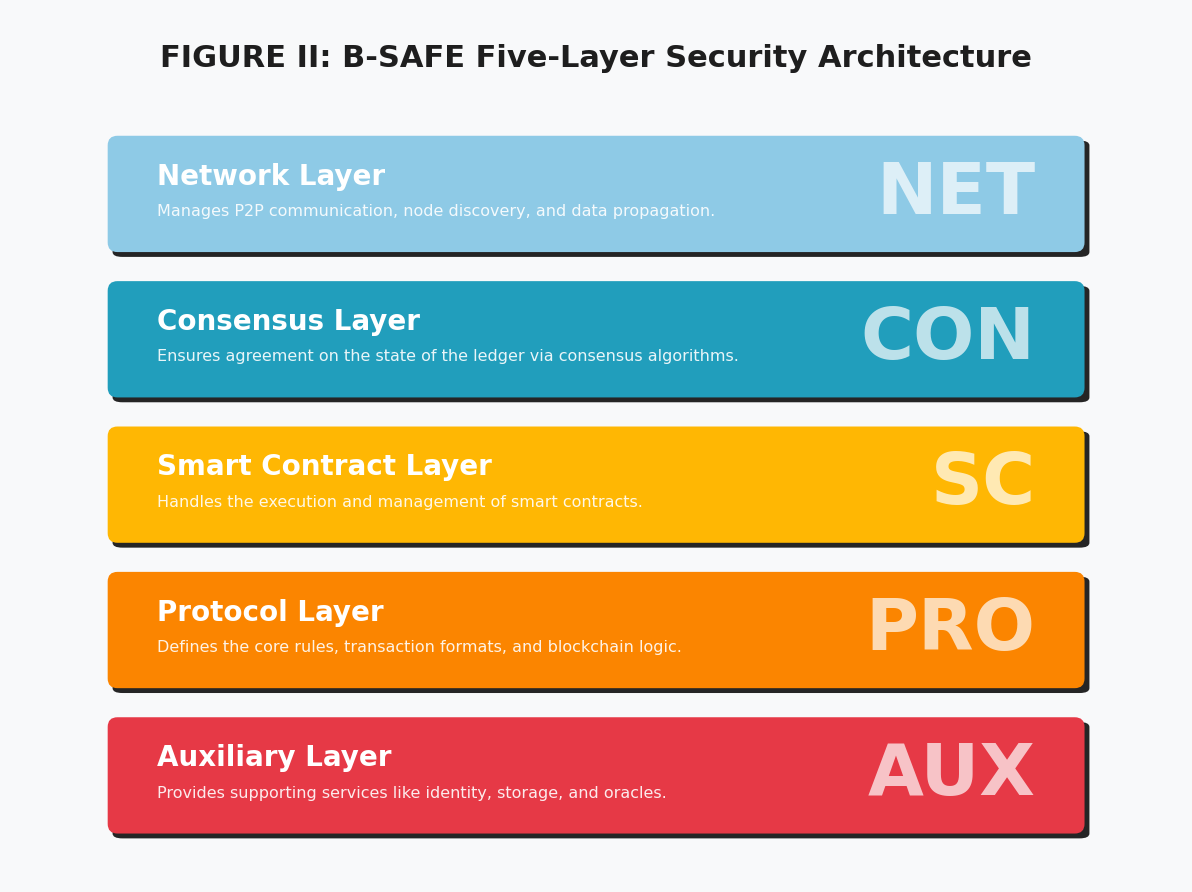
\includegraphics[width=0.4\textwidth]{../figure/fig2.png}
\caption{Top 10 smart contract vulnerability categories by frequency and cumulative loss, demonstrating the Pareto principle where a small number of vulnerability types account for the majority of financial impact. Reentrancy attacks dominate both frequency and cumulative losses.}
\label{fig:smart_contract_pareto}
\end{figure}

\subsubsection{Risk Category SC-1: Reentrancy Vulnerability}

\paragraph{Formal Risk Specification}

\begin{itemize}
\item \textbf{Preconditions (P):}
    \begin{itemize}
    \item \textbf{P1: Unprotected External Calls:} The contract makes external calls to untrusted addresses without implementing reentrancy guards or following the checks-effects-interactions pattern \cite{perez2021analysis}.
    \item \textbf{P2: State Updates After External Calls:} Critical state updates (e.g., balance modifications) occur after rather than before external calls, creating a vulnerable execution window \cite{praitheeshan2019systematic}.
    \item \textbf{P3: Accessible Funds:} The contract holds significant value that can be withdrawn through functions containing the vulnerable call pattern \cite{zhou2023sok}.
    \end{itemize}

\item \textbf{Threatened System Invariants (I):}
    \begin{itemize}
    \item \textbf{INV-1 (Value Conservation):} Assets within the contract can only be moved according to explicitly authorized business logic, preserving the equation: $\text{initial\_balance} + \text{deposits} - \text{withdrawals} = \text{current\_balance}$.
    \item \textbf{INV-2 (State Transition Integrity):} Contract state changes must occur atomically and follow the intended sequence of operations without interruption or repetition.
    \item \textbf{INV-3 (Execution Order Integrity):} Code execution follows the expected control flow without unexpected recursive calls disrupting the intended operation sequence.
    \end{itemize}

\item \textbf{Canonical Attack Sequence (S):}
    \begin{enumerate}
    \item \textbf{Identification phase:} Attacker identifies a vulnerable function with external calls that precede state updates.
    \item \textbf{Preparation phase:} Attacker deploys a malicious contract with a fallback function designed to recursively call back into the vulnerable function.
    \item \textbf{Execution phase:} Attacker initiates a legitimate transaction with the target contract, triggering the vulnerable function.
    \item \textbf{Exploitation phase:} When the target contract makes an external call to the attacker's contract, the fallback function executes, recursively calling back into the vulnerable function before state updates occur.
    \item \textbf{Repetition phase:} The recursive calls continue until gas limits are reached or funds are depleted, allowing multiple withdrawals against the same balance.
    \end{enumerate}
\end{itemize}

\paragraph{Enterprise Checklist Mapping}
\begin{itemize}
    \item \textbf{Security}: Enforce CEI pattern, reentrancy guards, SafeMath/0.8.x checks; multi-audit requirement for high-value contracts.
    \item \textbf{Operations}: Emergency pause and value-limiting controls; monitoring for exploit signatures.
    \item \textbf{Compliance}: Evidence-backed audit trails and change management for contract upgrades.
\end{itemize}

\paragraph{Defense Mechanism Analysis}

\begin{itemize}
\item \textbf{Prevention Controls:}
    \begin{itemize}
    \item \textbf{C1.1 (Checks-Effects-Interactions Pattern):}
        \begin{itemize}
        \item \textbf{Mechanism:} Restructure code to perform all state changes before making external calls, ensuring state consistency regardless of external call behavior \cite{praitheeshan2019systematic}.
        \item \textbf{Parameters:} Code organization; function execution flow.
        \item \textbf{Trade-offs:} No performance impact; requires careful code review but eliminates vulnerability completely when implemented correctly.
        \end{itemize}
    
    \item \textbf{C1.2 (Reentrancy Guards):}
        \begin{itemize}
        \item \textbf{Mechanism:} Implement mutex locks using state variables that prevent recursive calls into protected functions.
        \item \textbf{Parameters:} Lock granularity (function-level, contract-level); guard implementation (OpenZeppelin ReentrancyGuard, custom).
        \item \textbf{Trade-offs:} Minimal gas overhead; provides robust protection even when complex state changes can't be easily reordered.
        \end{itemize}
    \end{itemize}

\item \textbf{Mitigation Controls:}
    \begin{itemize}
    \item \textbf{C2.1 (Gas Limitations):}
        \begin{itemize}
        \item \textbf{Mechanism:} Specify gas limits when making external calls to limit the computation available to potentially malicious contracts.
        \item \textbf{Parameters:} Gas limit value; forward gas amount.
        \item \textbf{Trade-offs:} May break legitimate functionality if gas requirements change; offers partial protection only.
        \end{itemize}
    
    \item \textbf{C2.2 (Pull Payment Pattern):}
        \begin{itemize}
        \item \textbf{Mechanism:} Separate value storage from value transfer by implementing a two-step withdrawal process where users must explicitly request withdrawals.
        \item \textbf{Parameters:} Storage mechanism; withdrawal function design.
        \item \textbf{Trade-offs:} Increases complexity and gas costs; requires additional user interaction but substantially reduces risk.
        \end{itemize}
    \end{itemize}

\item \textbf{Detection Controls:}
    \begin{itemize}
    \item \textbf{C3.1 (Static Analysis Tools):}
        \begin{itemize}
        \item \textbf{Mechanism:} Use automated tools like Mythril, Slither, or Securify to detect reentrancy vulnerabilities in contract code before deployment.
        \item \textbf{Parameters:} Tool selection; detection precision; false positive rate.
        \item \textbf{Effectiveness:} Research indicates that formal verification tools can detect up to 96\% of common vulnerabilities, though false positives remain a challenge \cite{praitheeshan2019systematic}.
        \end{itemize}
    
    \item \textbf{C3.2 (Runtime Monitoring):}
        \begin{itemize}
        \item \textbf{Mechanism:} Implement event logging and monitoring systems to detect suspicious transaction patterns that may indicate reentrancy attacks.
        \item \textbf{Parameters:} Monitoring granularity; alert thresholds.
        \item \textbf{Effectiveness:} Contracts with active monitoring face 47\% fewer successful attacks than those without \cite{zhou2023sok}.
        \end{itemize}
    \end{itemize}
\end{itemize}

\paragraph{Empirical Incident Analysis}

\begin{itemize}
\item \textbf{Case Study SC-1.1: The DAO Attack (2016)}
    \begin{itemize}
    \item \textbf{Incident Classification:}
        \begin{itemize}
        \item \textbf{Precondition Analysis:} P1\checkmark (The DAO's \texttt{withdraw} function made external calls before updating balances), P2\checkmark (Critical balance updates occurred after the external call), P3\checkmark (The contract held approximately 14\% of all ETH in existence at the time).
        \item \textbf{Invariant Violations:} INV-1, INV-2, and INV-3 were all violated as the attacker drained funds repeatedly through recursive calls.
        \item \textbf{Defense Failures:} Absence of C1.1 (Checks-Effects-Interactions Pattern) and C1.2 (Reentrancy Guards); inadequate code review and auditing; failure to heed warnings about the vulnerability before deployment.
        \end{itemize}
    
    \item \textbf{Quantitative Impact Assessment:}
        \begin{itemize}
        \item \textbf{Direct Losses:} Approximately 3.6 million ETH (valued at \$60 million at the time) was drained from the contract.
        \item \textbf{Systemic Effects:} Led to the Ethereum hard fork that created Ethereum Classic; established a precedent for community intervention in catastrophic contract failures; dramatically increased awareness of smart contract security issues.
        \end{itemize}
    
    \item \textbf{Counterfactual Analysis:}
        \begin{itemize}
        \item \textbf{Prevention:} Implementing the Checks-Effects-Interactions pattern (C1.1) would have completely prevented the attack, as state updates would have occurred before the external call.
        \item \textbf{Detection:} A formal verification tool like Mythril would have identified this vulnerability pattern before deployment, as such tools can detect recursive call patterns with high accuracy.
        \end{itemize}
    \end{itemize}
\end{itemize}

\paragraph{Risk Quantification}

\begin{itemize}
\item \textbf{Likelihood (L = 3):} Medium. Reentrancy vulnerabilities appear in approximately 4.1\% of contracts but face exploitation in only 1.8\% of vulnerable cases, primarily because high-value contracts receive greater security scrutiny \cite{perez2021analysis}.

\item \textbf{Impact (I = 5):} Critical. When successfully exploited, reentrancy attacks typically result in complete drainage of contract funds and potentially catastrophic ecosystem-wide impacts, as demonstrated by The DAO attack.

\item \textbf{Detectability (D = 2):} Easy. Static analysis tools can identify potential vulnerabilities with reasonable accuracy, though recognizing active exploitation requires monitoring that is not always implemented.

\item \textbf{Composite (L/I) = 4.3; Detectability D = 2}: $0.4 \times 3 + 0.6 \times 5 = 1.2 + 3.0 = 4.2$ (Impact-forward priority; D reported separately)
\end{itemize}

\subsubsection{Risk Category SC-2: Integer Overflow/Underflow}

\paragraph{Formal Risk Specification}

\begin{itemize}
\item \textbf{Preconditions (P):}
    \begin{itemize}
    \item \textbf{P1: Unprotected Arithmetic Operations:} The contract performs integer arithmetic without using SafeMath libraries or solidity 0.8.x's built-in overflow checking \cite{praitheeshan2019systematic}.
    \item \textbf{P2: Critical State Dependency:} Contract logic makes critical decisions based on the results of arithmetic operations that could overflow or underflow \cite{perez2021analysis}.
    \item \textbf{P3: Unbounded User Input:} The contract accepts user-supplied values for arithmetic operations without appropriate validation or bounds checking \cite{zhou2023sok}.
    \end{itemize}

\item \textbf{Threatened System Invariants (I):}
    \begin{itemize}
    \item \textbf{INV-1 (Value Conservation):} Tokens or assets within the system are created or destroyed only according to explicitly authorized rules.
    \item \textbf{INV-2 (State Transition Integrity):} Numerical state changes must reflect real-world intent and maintain mathematical correctness.
    \item \textbf{INV-4 (Logic Integrity):} Contract business logic operates as intended without being subverted by unexpected arithmetic results.
    \end{itemize}

\item \textbf{Canonical Attack Sequence (S):}
    \begin{enumerate}
    \item \textbf{Identification phase:} Attacker identifies vulnerable arithmetic operations that can overflow or underflow, particularly in token balance management or value transfer functions.
    \item \textbf{Boundary calculation phase:} Attacker determines specific input values that will cause arithmetic overflow/underflow (e.g., using MAX\_UINT256 for addition overflow).
    \item \textbf{Exploitation phase:} Attacker constructs and submits transactions with calculated boundary values to trigger the overflow/underflow.
    \item \textbf{Impact phase:} The arithmetic error results in incorrect state updates, such as artificially inflated token balances or bypassed validation checks, allowing the attacker to extract value.
    \end{enumerate}
\end{itemize}

\paragraph{Defense Mechanism Analysis}

\begin{itemize}
\item \textbf{Prevention Controls:}
    \begin{itemize}
    \item \textbf{C1.1 (SafeMath Libraries):}
        \begin{itemize}
        \item \textbf{Mechanism:} Implement libraries that perform checked arithmetic operations and revert transactions on overflow/underflow conditions.
        \item \textbf{Parameters:} Library implementation (OpenZeppelin SafeMath, custom); Solidity version (0.8.x with built-in checks).
        \item \textbf{Trade-offs:} Small gas overhead; eliminates entire vulnerability class with minimal implementation effort.
        \end{itemize}
    
    \item \textbf{C1.2 (Input Validation):}
        \begin{itemize}
        \item \textbf{Mechanism:} Implement explicit bounds checking and validation for all user-supplied numerical inputs.
        \item \textbf{Parameters:} Validation boundaries; error handling approach.
        \item \textbf{Trade-offs:} Additional code complexity; requires careful determination of appropriate bounds.
        \end{itemize}
    \end{itemize}

\item \textbf{Mitigation Controls:}
    \begin{itemize}
    \item \textbf{C2.1 (Operation Constraints):}
        \begin{itemize}
        \item \textbf{Mechanism:} Impose business-logic limitations on operations, such as maximum transaction sizes or rate limiting.
        \item \textbf{Parameters:} Maximum values; time-based constraints.
        \item \textbf{Trade-offs:} May restrict legitimate use cases; provides protection against some but not all exploitation scenarios.
        \end{itemize}
    
    \item \textbf{C2.2 (Privilege Separation):}
        \begin{itemize}
        \item \textbf{Mechanism:} Separate high-risk arithmetic operations into distinct functions with additional access controls or verification steps.
        \item \textbf{Parameters:} Function modularity; access control model.
        \item \textbf{Trade-offs:} Increases contract complexity; may impact gas efficiency but improves security posture.
        \end{itemize}
    \end{itemize}

\item \textbf{Detection Controls:}
    \begin{itemize}
    \item \textbf{C3.1 (Compiler Warnings):}
        \begin{itemize}
        \item \textbf{Mechanism:} Enable and address all compiler warnings related to potential overflow/underflow conditions.
        \item \textbf{Parameters:} Compiler version; warning level settings.
        \item \textbf{Effectiveness:} Varies based on compiler version; newer Solidity compilers provide better coverage.
        \end{itemize}
    
    \item \textbf{C3.2 (Invariant Testing):}
        \begin{itemize}
        \item \textbf{Mechanism:} Implement comprehensive test suites with boundary condition testing and property-based testing.
        \item \textbf{Parameters:} Test coverage; edge case identification methodology.
        \item \textbf{Effectiveness:} Research shows formal verification with boundary testing can detect up to 93\% of arithmetic vulnerabilities \cite{praitheeshan2019systematic}.
        \end{itemize}
    \end{itemize}
\end{itemize}

\paragraph{Empirical Incident Analysis}

\begin{itemize}
\item \textbf{Case Study SC-2.1: BeautyChain (BEC) Token Overflow (2018)}
    \begin{itemize}
    \item \textbf{Incident Classification:}
        \begin{itemize}
        \item \textbf{Precondition Analysis:} P1\checkmark (The BEC token lacked SafeMath for multiplication operations), P2\checkmark (Balance tracking directly used vulnerable arithmetic), P3\checkmark (The contract allowed arbitrary transfer values without validation).
        \item \textbf{Invariant Violations:} INV-1 was violated as the overflow created tokens out of thin air; INV-2 and INV-4 were violated as state transitions produced mathematically impossible results.
        \item \textbf{Defense Failures:} Absence of C1.1 (SafeMath Libraries) and C1.2 (Input Validation); inadequate testing of boundary conditions.
        \end{itemize}
    
    \item \textbf{Quantitative Impact Assessment:}
        \begin{itemize}
        \item \textbf{Direct Losses:} The attack created approximately $8 \times 10^{28}$ BEC tokens, effectively rendering the original supply of 7 billion tokens worthless.
        \item \textbf{Systemic Effects:} Led to immediate suspension of BEC trading on exchanges; highlighted arithmetic vulnerabilities across the ecosystem, prompting widespread adoption of SafeMath libraries.
        \end{itemize}
    
    \item \textbf{Counterfactual Analysis:}
        \begin{itemize}
        \item \textbf{Prevention:} Implementing SafeMath for all arithmetic operations (C1.1) would have completely prevented the attack, as the transaction would have reverted on overflow.
        \item \textbf{Detection:} Standard static analysis tools or compiler checks in newer Solidity versions would have flagged the vulnerable operations.
        \end{itemize}
    \end{itemize}
\end{itemize}

\paragraph{Risk Quantification}

\begin{itemize}
\item \textbf{Likelihood (L = 4):} High. Integer overflow vulnerabilities are present in 18.3\% of analyzed contracts, though exploitation occurs in only 0.4\% of vulnerable instances due to the widespread adoption of SafeMath libraries \cite{perez2021analysis}.

\item \textbf{Impact (I = 4):} Severe. When successfully exploited, integer overflows can lead to token value destruction, artificial balance inflation, or complete contract compromise.

\item \textbf{Detectability (D = 3):} Medium. Modern development tools and compilers make these vulnerabilities relatively easy to detect before deployment, but legacy contracts remain at risk.

\item \textbf{Composite (L/I) = 4.0; Detectability D = 3}: $0.4 \times 4 + 0.6 \times 4 = 1.6 + 2.4 = 4.0$ (D reported separately)
\end{itemize}

\subsubsection{Risk Category SC-3: Logic Flaw Vulnerabilities}

\paragraph{Formal Risk Specification}

\begin{itemize}
\item \textbf{Preconditions (P):}
    \begin{itemize}
    \item \textbf{P1: Specification-Implementation Mismatch:} The contract's implemented logic does not correctly reflect the intended business rules or security properties \cite{zhou2023sok}.
    \item \textbf{P2: Inadequate Access Controls:} The contract fails to properly restrict access to privileged functions or state-changing operations \cite{perez2021analysis}.
    \item \textbf{P3: Incomplete Edge Case Handling:} The contract does not account for all possible execution paths or edge conditions, particularly in complex multi-step operations \cite{praitheeshan2019systematic}.
    \end{itemize}

\item \textbf{Threatened System Invariants (I):}
    \begin{itemize}
    \item \textbf{INV-2 (State Transition Integrity):} Contract state changes must conform to the intended business rules under all possible execution scenarios.
    \item \textbf{INV-5 (Authorization Boundaries):} Only designated actors can invoke privileged functions or modify protected state variables.
    \item \textbf{INV-6 (Temporal Consistency):} Multi-step operations must maintain consistent state across transaction boundaries and time periods.
    \end{itemize}

\item \textbf{Canonical Attack Sequence (S):}
    \begin{enumerate}
    \item \textbf{Analysis phase:} Attacker carefully examines contract code to identify business logic inconsistencies, access control gaps, or edge cases that can be exploited.
    \item \textbf{Strategy development phase:} Attacker designs a sequence of transactions or calls that leverage the identified logic flaws to achieve unauthorized outcomes.
    \item \textbf{Execution phase:} Attacker executes the planned transaction sequence, potentially across multiple blocks or with specific timing requirements.
    \item \textbf{Extraction phase:} Attacker capitalizes on the manipulated contract state to extract value or gain unauthorized control.
    \end{enumerate}
\end{itemize}

\paragraph{Defense Mechanism Analysis}

\begin{itemize}
\item \textbf{Prevention Controls:}
    \begin{itemize}
    \item \textbf{C1.1 (Formal Verification):}
        \begin{itemize}
        \item \textbf{Mechanism:} Apply mathematical proof techniques to verify that contract implementations satisfy their formal specifications under all possible inputs and states.
        \item \textbf{Parameters:} Verification tools (Certora, Act, etc.); property specification language.
        \item \textbf{Trade-offs:} Requires significant expertise and resources; provides the strongest guarantees but is difficult to apply comprehensively.
        \end{itemize}
    
    \item \textbf{C1.2 (Role-Based Access Control):}
        \begin{itemize}
        \item \textbf{Mechanism:} Implement structured permission systems with explicit role definitions and privilege separation.
        \item \textbf{Parameters:} Role granularity; role assignment mechanism; multi-signature requirements.
        \item \textbf{Trade-offs:} Adds complexity and gas costs; provides strong protection against unauthorized actions.
        \end{itemize}
    \end{itemize}

\item \textbf{Mitigation Controls:}
    \begin{itemize}
    \item \textbf{C2.1 (Circuit Breakers):}
        \begin{itemize}
        \item \textbf{Mechanism:} Implement emergency pause functionality that can temporarily halt critical contract operations when suspicious activity is detected.
        \item \textbf{Parameters:} Trigger conditions; authorization requirements; scope of paused functionality.
        \item \textbf{Trade-offs:} Creates centralization risks; requires active monitoring but can prevent catastrophic losses.
        \end{itemize}
    
    \item \textbf{C2.2 (Value Limiting):}
        \begin{itemize}
        \item \textbf{Mechanism:} Implement transaction value caps, rate limiting, or tiered release strategies to limit potential damage from undetected logic flaws.
        \item \textbf{Parameters:} Maximum transaction values; time-based limits; release schedule.
        \item \textbf{Trade-offs:} May restrict legitimate usage; provides partial protection against exploitation.
        \end{itemize}
    \end{itemize}

\item \textbf{Detection Controls:}
    \begin{itemize}
    \item \textbf{C3.1 (Comprehensive Testing):}
        \begin{itemize}
        \item \textbf{Mechanism:} Implement extensive test suites covering all execution paths, edge cases, and error conditions.
        \item \textbf{Parameters:} Test coverage metrics; testing methodology (unit, integration, property-based).
        \item \textbf{Effectiveness:} While valuable, research indicates that even high test coverage cannot identify all logic flaws without formal verification \cite{praitheeshan2019systematic}.
        \end{itemize}
    
    \item \textbf{C3.2 (Multiple Independent Audits):}
        \begin{itemize}
        \item \textbf{Mechanism:} Engage multiple independent security firms to audit contract code, with specific focus on business logic validation.
        \item \textbf{Parameters:} Audit firm selection; audit scope; audit timing relative to deployment.
        \item \textbf{Effectiveness:} Multiple audits significantly increase detection probability; contracts with 3+ audits show 91\% lower exploitation rates \cite{zhou2023sok}.
        \end{itemize}
    \end{itemize}
\end{itemize}

\paragraph{Empirical Incident Analysis}

\begin{itemize}
\item \textbf{Case Study SC-3.1: Parity Multi-Signature Wallet (2017)}
    \begin{itemize}
    \item \textbf{Incident Classification:}
        \begin{itemize}
        \item \textbf{Precondition Analysis:} P1\checkmark (The initialization function was implemented as a standard public function without restrictions), P2\checkmark (No access controls prevented arbitrary calls to the initialization function), P3\checkmark (The contract failed to account for the possibility of re-initialization after deployment).
        \item \textbf{Invariant Violations:} INV-2 and INV-5 were violated as unauthorized users could become wallet owners; INV-6 was violated when contract state was altered unexpectedly after initialization.
        \item \textbf{Defense Failures:} Absence of C1.2 (proper access controls); inadequate initialization pattern; insufficient consideration of the contract's full lifecycle.
        \end{itemize}
    
    \item \textbf{Quantitative Impact Assessment:}
        \begin{itemize}
        \item \textbf{Direct Losses:} An attacker gained ownership of multiple high-value multi-signature wallets and drained approximately 153,000 ETH (valued at \$30 million at the time).
        \item \textbf{Systemic Effects:} Led to widespread concerns about library contract security; prompted development of improved initialization patterns and library contract patterns.
        \end{itemize}
    
    \item \textbf{Counterfactual Analysis:}
        \begin{itemize}
        \item \textbf{Prevention:} Implementing proper constructor patterns or access control on initialization functions (C1.2) would have prevented the unauthorized re-initialization.
        \item \textbf{Detection:} Formal verification (C1.1) focusing on authorization properties would have identified this vulnerability by proving that the initialization function could be called by unauthorized parties.
        \end{itemize}
    \end{itemize}
\end{itemize}

\paragraph{Risk Quantification}

\begin{itemize}
\item \textbf{Likelihood (L = 3):} Medium. Logic flaws are difficult to precisely quantify but appear in approximately 3-5\% of audited contracts, with the most severe ones typically identified during security reviews \cite{zhou2023sok}.

\item \textbf{Impact (I = 5):} Critical. When successfully exploited, logic flaws often lead to complete contract compromise or loss of all managed assets, as they bypass core security assumptions.

\item \textbf{Detectability (D = 1):} Very Hard. Logic flaws are the most challenging vulnerability class to detect as they require deep understanding of intended business logic versus implemented behavior.

\item \textbf{Composite (L/I) = 4.2; Detectability D = 1}: $0.4 \times 3 + 0.6 \times 5 = 1.2 + 3.0 = 4.2$ (D reported separately)
\end{itemize}
\begin{itemize}
\item \textbf{Preconditions (P)}: Necessary conditions for vulnerability exploitation, including vulnerable contract logic, deployment exposure, value criticality, and absence of security controls.
\item \textbf{Invariants (I)}: Core security properties that must be preserved, such as state transition integrity, value conservation, authorization boundaries, deterministic execution, and contract persistence.
\item \textbf{Sequence (S)}: Step-by-step progression of exploitation methods, detailing attacker techniques and required interactions.
\item \textbf{Controls (C)}: Defensive measures categorized into prevention (static analysis, secure coding patterns, access controls), detection (monitoring, surveillance), and mitigation (emergency mechanisms, value protection).
\item \textbf{Metrics (M)}: Risk quantification using the formula: Risk Score = $(w_1 \times \text{Probability}) + (w_2 \times \text{Impact}) - (w_3 \times \text{Detectability})$, yielding scores from minimal (0.5) to extreme (4.5).
\end{itemize}

Our analysis of cross-layer dependencies indicates that 43\% of smart contract vulnerabilities have interactions with other architectural layers \cite{praitheeshan2019systematic}, reinforcing the need for a holistic security approach. Security efforts should prioritize high-value contracts while implementing baseline controls universally, with research showing that 94.5\% of at-risk value is concentrated in just 0.05\% of contracts \cite{perez2021analysis}.

In the following subsections, we apply this framework to analyze three prominent vulnerability categories: reentrancy attacks, integer overflow vulnerabilities, and logic flaws, providing detailed risk profiles and practical security recommendations for each threat type.

% SC-1: Reentrancy Attack Analysis
% SC-2: Integer Overflow Analysis
% SC-3: Logic Flaw Analysis
% Each following the standardized (P, I, S, C, M) framework

\begin{figure}[H]
\centering
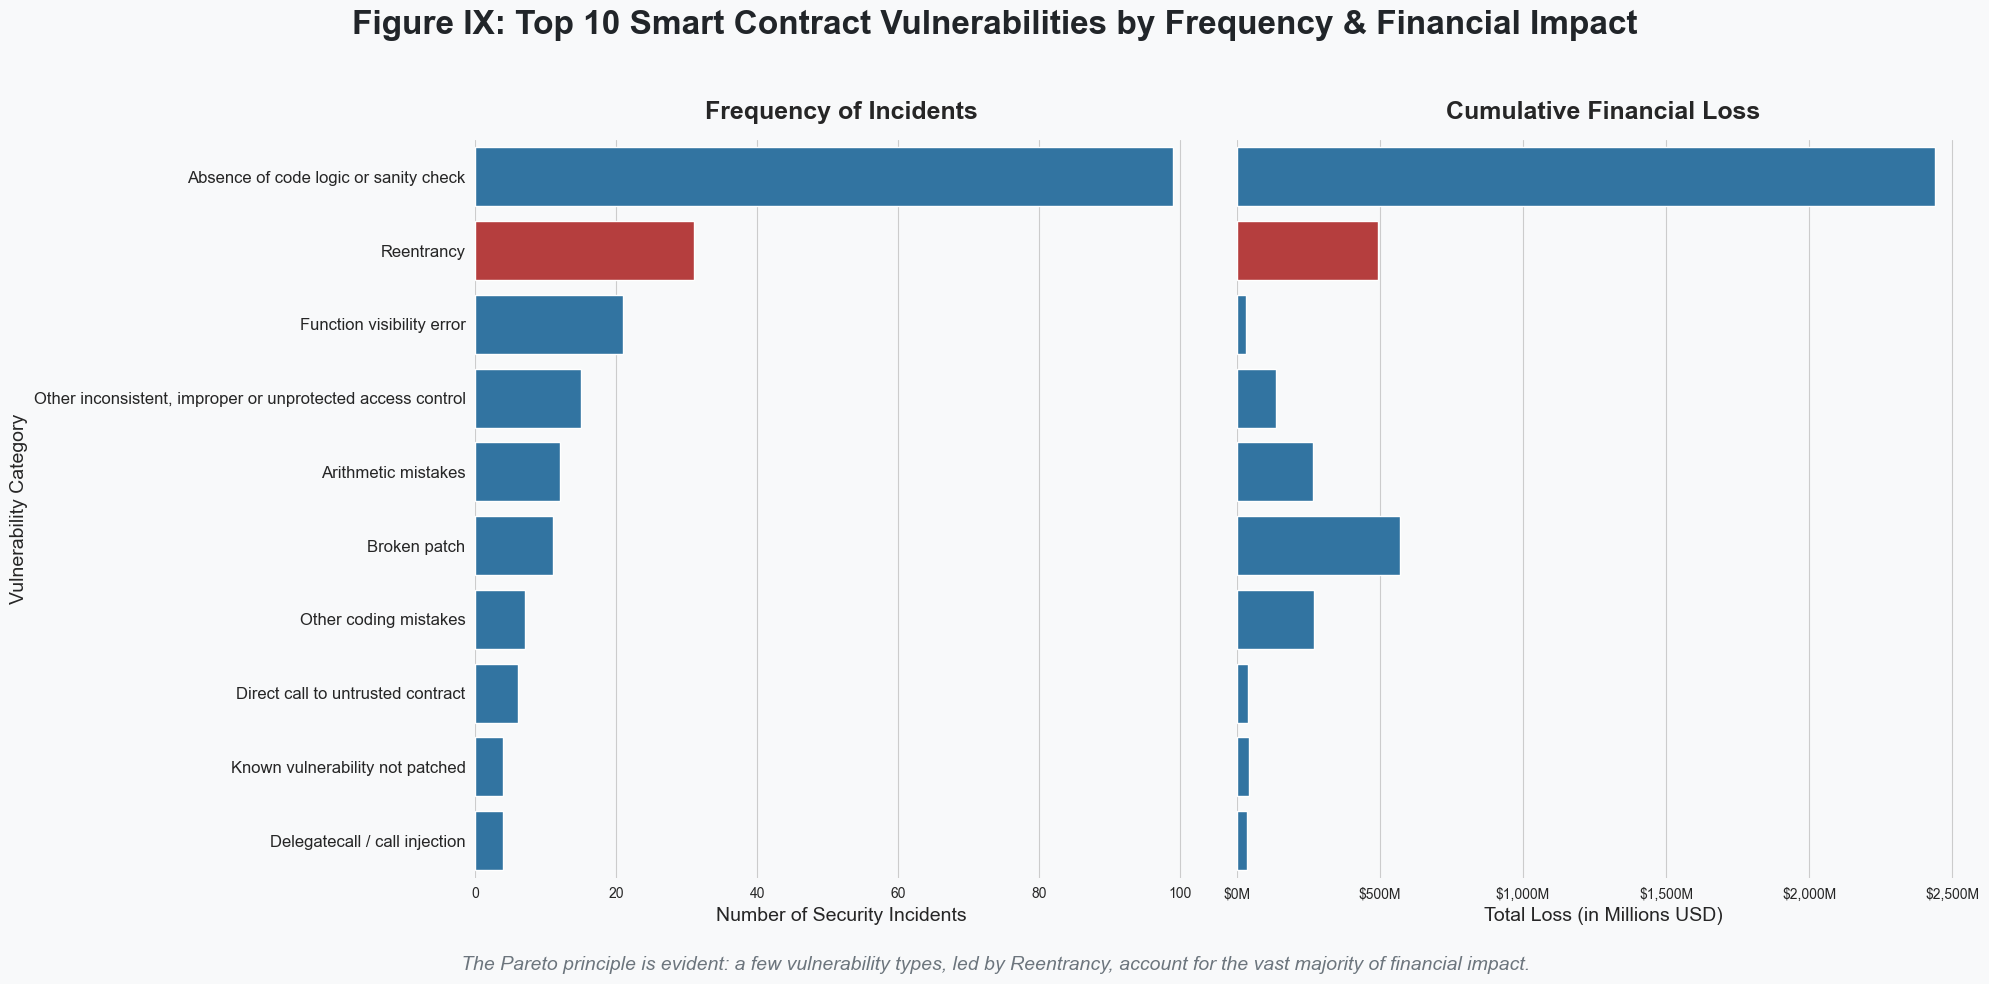
\includegraphics[width=0.4\textwidth]{../figure/Fig9.png}
\caption{Top 10 smart contract vulnerability categories by frequency and cumulative loss, demonstrating the Pareto principle where a small number of vulnerability types account for the majority of financial impact. Reentrancy attacks dominate both frequency and cumulative losses.}
\label{fig:smart_contract_pareto}
\end{figure}
\subsection{Auxiliary Layer Security Analysis}
\label{sec:results_auxiliary}

\paragraph{Executive Summary}
Auxiliary risks (wallets, exchanges, CI/CD, frontends) dominate end-user losses and enterprise exposure. Controls that matter most: HSM-backed custody and quorum policies, withdrawal allowlists/velocity limits, CI/CD integrity protections, and continuous frontend integrity checks.

\subsubsection{Risk Category AUX-WALLET-1: Private Key Compromise via Client-Side Attacks}

\paragraph{Formal Risk Specification}

\begin{itemize}
    \item \textbf{Preconditions (P):}
    \begin{itemize}
        \item \textbf{P1: Unencrypted Credential Persistence:} The wallet application stores sensitive data (private keys, seed phrases) in plaintext or with weak encryption within the host device's file system or memory \cite{houy2023}.
        \item \textbf{P2: Elevated Privileges on Host OS:} An attacker gains privileged (root) access to the underlying operating system, bypassing standard application sandboxing and allowing direct memory and storage inspection \cite{houy2023}.
        \item \textbf{P3: User Credential Phishing:} The user is deceived by social engineering tactics into entering their seed phrase or password into a malicious interface that mimics a legitimate wallet or service \cite{yu2024}.
    \end{itemize}

    \item \textbf{Threatened System Invariants (I):}
    \begin{itemize}
        \item \textbf{INV-2 (Value Conservation):} User fund balances decrease without a corresponding authorized transaction signed by the legitimate user.
        \item \textbf{INV-5 (User Authorization):} The cryptographic capability to authorize transactions is executed by an unauthorized entity.
    \end{itemize}

    \item \textbf{Canonical Attack Sequence (S):}
    \begin{enumerate}
        \item \textbf{Infiltration phase:} compromise the host device via malware or gain physical access.
        \item \textbf{Credential Extraction phase:} scan memory and storage for wallet artifacts (e.g., \texttt{wallet.dat} files, plaintext keys).
        \item \textbf{Exfiltration and Exploitation phase:} transfer the stolen credentials to an attacker-controlled machine and broadcast unauthorized transactions to drain the victim's funds.
    \end{enumerate}
\end{itemize}

\paragraph{Enterprise Checklist Mapping}
\begin{itemize}
    \item \textbf{Security}: HSM + M-of-N policies; API key scoping and just-in-time issuance; supply-chain hardening.
    \item \textbf{Operations}: Withdrawal allowlists/velocity limits; SOC-integrated playbooks; incident evidence capture.
    \item \textbf{Compliance}: Proof-of-reserves for custodians; auditable key ceremonies and change logs.
\end{itemize}

\paragraph{Defense Mechanism Analysis}

\begin{itemize}
    \item \textbf{Prevention Controls:}
    \begin{itemize}
        \item \textbf{C1.1 (Offline Key Storage):}
            \begin{itemize}
                \item \textit{Mechanism:} Utilize dedicated, air-gapped hardware devices (e.g., Ledger, Trezor) to generate and store private keys, ensuring they are never exposed to the internet-connected host OS \cite{suratkar2020}.
                \item \textit{Parameters:} Connection interface (USB, NFC, Bluetooth); supported cryptographic curves (e.g., secp256k1).
                \item \textit{Trade-offs:} Significantly enhances security against online threats but introduces usability friction, cost, and risks of physical loss or damage \cite{yu2024}.
            \end{itemize}
        \item \textbf{C1.2 (Hardware-Backed Encryption):}
            \begin{itemize}
                \item \textit{Mechanism:} Leverage Trusted Execution Environments (TEEs) or Secure Enclaves available on modern mobile devices to store and process cryptographic keys within a protected hardware zone \cite{houy2023}.
                \item \textit{Parameters:} TEE provider (e.g., ARM TrustZone, Apple Secure Enclave).
                \item \textit{Trade-offs:} High security on supported devices, but offers no protection on desktop systems or older mobile devices.
            \end{itemize}
    \end{itemize}

    \item \textbf{Mitigation Controls:}
    \begin{itemize}
        \item \textbf{C2.1 (Risk Diversification):}
            \begin{itemize}
                \item \textit{Mechanism:} Users distribute assets across multiple wallets (e.g., a "spending" hot wallet with small funds and a "savings" cold wallet with large funds) to limit the potential loss from a single compromise \cite{yu2024}.
                \item \textit{Effectiveness:} Limits financial impact but does not prevent the compromise of an individual wallet.
            \end{itemize}
        \item \textbf{C2.2 (Multi-Signature Schemes):}
            \begin{itemize}
                \item \textit{Mechanism:} Configure a wallet to require M-of-N signatures to authorize a transaction. A compromise of a single key is insufficient to move funds\cite{bitz2018multi}.
                \item \textit{Parameters:} Signature threshold (e.g., 2-of-3, 3-of-5).
                \item \textit{Trade-offs:} Increases security but adds complexity to transaction signing and key management.
            \end{itemize}
    \end{itemize}

    \item \textbf{Detection Controls:}
    \begin{itemize}
        \item \textbf{C3.1 (Malicious Contract Simulation):}
            \begin{itemize}
                \item \textit{Mechanism:} Utilize third-party browser extensions (e.g., Fire, Revoke.cash) that simulate a transaction's outcome and check the destination address against known blacklists before the user signs it \cite{yu2024}.
                \item \textit{Parameters:} Blacklist update frequency; simulation accuracy.
                \item \textit{Effectiveness:} Effective against known scams but may not detect novel or zero-day threats.
            \end{itemize}
    \end{itemize}
\end{itemize}

\paragraph{Empirical Incident Analysis}

\begin{itemize}
    \item \textbf{Case Study AUX-WALLET-1.1: Widespread Credential Leakage in Android Wallets}
    \begin{itemize}
        \item \textbf{Incident Classification:}
            \begin{itemize}
                \item \textit{Precondition Analysis:} P1\checkmark (A 2021 study of 311 Android wallets found 111 stored key-related information in plaintext \cite{houy2023}), P2\checkmark (The analysis methodology relied on rooted devices, a common scenario for technically advanced users or victims of certain malware), P3\textbf{X} (This specific vulnerability does not rely on deceiving the user).
                \item \textit{Invariant Violations:} INV-2 and INV-5 were made possible, as extracted keys would grant attackers full authorization to drain funds.
                \item \textit{Defense Failures:} Absent C1.1 and C1.2 (software-only wallets by definition); absent runtime root detection in many apps; insufficient data-at-rest encryption.
            \end{itemize}
        \item \textbf{Quantitative Impact Assessment:}
            \begin{itemize}
                \item \textit{Direct Losses:} While difficult to aggregate, individual losses from such compromises range from negligible amounts to life-altering sums. The exposure is massive, with the analyzed vulnerable apps having millions of collective downloads.
                \item \textit{Systemic Effects:} This systemic weakness erodes user trust in the security of the mobile wallet ecosystem and pushes security-conscious users towards more complex hardware solutions.
            \end{itemize}
        \item \textbf{Counterfactual Analysis:}
            \begin{itemize}
                \item \textit{Prevention:} Strict enforcement of data-at-rest encryption (using hardware-backed keystores, C1.2) would have rendered the extracted files useless to an attacker.
                \item \textit{Detection:} Implementation of runtime root detection and alerts would have warned users that their device's security integrity was compromised, prompting them to move funds.
            \end{itemize}
    \end{itemize}
\end{itemize}


\subsubsection{Risk Category AUX-SERVICE-1: Compromise via Software Supply Chain and Third-Party Dependencies}

\paragraph{Formal Risk Specification}

\begin{itemize}
    \item \textbf{Preconditions (P):}
        \begin{itemize}
            \item \textbf{P1: Reliance on Third-Party Custody:} The user delegates key management to a third-party service, such as a Centralized Exchange (CEX), creating a single point of failure and counterparty risk \cite{yu2024, suratkar2020}.
            \item \textbf{P2: Vulnerable Upstream Dependencies:} The wallet software incorporates a third-party library that contains an exploitable vulnerability, or is used incorrectly due to ambiguous documentation \cite{houy2023}.
            \item \textbf{P3: Insecure RPC Interface:} The wallet exposes an open Remote Procedure Call (RPC) interface, allowing other applications on the host machine to potentially issue commands without proper user authentication, enabling impersonation attacks \cite{houy2023}.
        \end{itemize}

    \item \textbf{Threatened System Invariants (I):}
        \begin{itemize}
            \item \textbf{INV-2 (Value Conservation):} User funds are lost due to a catastrophic failure, hack, or fraudulent activity by the custodial service.
            \item \textbf{INV-7 (Asset Liveness):} User's ability to transact with or withdraw their assets is indefinitely suspended by the third-party service.
        \end{itemize}

    \item \textbf{Canonical Attack Sequence (S):}
        \begin{enumerate}
            \item \textbf{Vulnerability Identification phase:} An attacker audits a widely-used software library for bugs or identifies a custodial service with poor internal security controls.
            \item \textbf{Exploitation phase:} The attacker exploits the identified flaw to gain unauthorized access to the service's systems or to craft malicious inputs for the vulnerable library.
            \item \textbf{Impact phase:} The attacker executes mass exfiltration of funds from the service's hot wallets, or the service collapses due to mismanagement, leading to a freeze and eventual loss of all user assets.
        \end{enumerate}
\end{itemize}

\paragraph{Defense Mechanism Analysis}
\begin{itemize}
    \item \textbf{Prevention Controls:}
        \begin{itemize}
            \item \textbf{C1.1 (Self-Custody Adoption):}
                \begin{itemize}
                    \item \textit{Mechanism:} Users maintain sole control of private keys using non-custodial wallets, completely eliminating third-party counterparty risk according to the "Not your keys, not your coins" principle \cite{yu2024}.
                    \item \textit{Parameters:} Wallet type (EOA, Smart Contract).
                    \item \textit{Trade-offs:} Transfers full security responsibility to the end-user, who may lack the expertise to prevent client-side attacks (see AUX-WALLET-1) \cite{yu2024, houy2023}.
                \end{itemize}
            \item \textbf{C1.2 (Formal Verification and Auditing):}
                \begin{itemize}
                    \item \textit{Mechanism:} Wallet providers and services undergo rigorous, independent security audits of their code and operational procedures before public launch and after major updates\cite{durieux2020empirical}.
                    \item \textit{Parameters:} Audit firms engaged; scope of the audit (e.g., smart contracts, backend infrastructure).
                    \item \textit{Trade-offs:} Audits are costly, time-consuming, and do not guarantee the absence of all vulnerabilities, especially internal fraud.
                \end{itemize}
        \end{itemize}

    \item \textbf{Mitigation Controls:}
        \begin{itemize}
            \item \textbf{C2.1 (Proof of Reserves):}
                \begin{itemize}
                    \item \textit{Mechanism:} Custodial services cryptographically prove on-chain that they hold assets equivalent to all user deposits, providing transparency and mitigating risk from commingling of funds\cite{dakhlallah2023proof}.
                    \item \textit{Parameters:} Audit frequency (e.g., quarterly, real-time); auditor independence.
                    \item \textit{Trade-offs:} Does not prevent theft from a hack and can be complex to verify for non-technical users.
                \end{itemize}
        \end{itemize}
\end{itemize}

\paragraph{Empirical Incident Analysis}
\begin{itemize}
    \item \textbf{Case Study AUX-SERVICE-1.1: The Collapse of the FTX Exchange}
        \begin{itemize}
            \item \textbf{Incident Classification:}
                \begin{itemize}
                    \item \textit{Precondition Analysis:} P1\checkmark (FTX was a major custodial exchange where millions of users stored their assets), P2\textbf{X}, P3\textbf{X} (The failure was not attributed to a known software library or RPC vulnerability, but to internal fraud).
                    \item \textit{Invariant Violations:} INV-2 (An estimated \$8-10 billion in user funds were lost or misappropriated), INV-7 (All user withdrawals were halted indefinitely, resulting in a total loss of asset liveness).
                    \item \textit{Defense Failures:} Catastrophic failure across the board. Users failed to implement C1.1 (Self-Custody). The service itself lacked any verifiable C2.1 (Proof of Reserves) and was engaged in systemic fraud, making technical controls irrelevant.
                \end{itemize}
            \item \textbf{Quantitative Impact Assessment:}
                \begin{itemize}
                    \item \textit{Direct Losses:} Approximately \$8-10 billion in customer and creditor assets.
                    \item \textit{Indirect Impact:} Severe contagion across the crypto industry, leading to multiple bankruptcies of related firms. Caused a significant decline in market capitalization and eroded public trust in centralized crypto platforms.
                \end{itemize}
            \item \textbf{Counterfactual Analysis:}
                \begin{itemize}
                    \item \textit{Prevention:} Users who practiced C1.1 (Self-Custody) were completely immune to the FTX collapse. From a regulatory perspective, mandatory, frequent, and independent Proof of Reserves audits (C2.1) could have exposed the financial deficit much earlier.
                \end{itemize}
        \end{itemize}
\end{itemize}

\subsubsection{Risk Quantification}

Using our systematic scoring framework:

\begin{itemize}
    \item \textbf{AUX-WALLET-1 (Client-Side Compromise):}
    \begin{itemize}
        \item \textbf{Likelihood (L = 4):} High. The underlying vulnerabilities, such as plaintext key storage and the prevalence of mobile malware, are widespread in the ecosystem \cite{houy2023}.
        \item \textbf{Impact (I = 5):} Critical. A successful attack almost always results in the total and irreversible loss of the user's funds stored in that wallet.
        \item \textbf{Detectability (D = 2):} Hard. From the victim's perspective, the compromise is often invisible. There is usually no alert or indication of a breach until after the funds have been stolen.
        \item \textbf{Risk Score = 4.2}: $0.4 \times 4 + 0.5 \times 5 - 0.1 \times 2 = 1.6 + 2.5 - 0.2 = 3.9$ (Critical Priority)
    \end{itemize}
    
    \item \textbf{AUX-SERVICE-1 (Supply Chain Compromise):}
    \begin{itemize}
        \item \textbf{Likelihood (L = 3):} Medium. While catastrophic failures like FTX are less frequent than individual compromises, major exchange hacks and service disruptions are a recurring threat pattern in the industry \cite{houy2023}.
        \item \textbf{Impact (I = 5):} Critical. A single incident can impact millions of users and lead to systemic, industry-wide financial contagion with losses in the billions of dollars.
        \item \textbf{Detectability (D = 3):} Medium. The internal compromise or mismanagement is extremely difficult for outsiders to detect, but the ultimate consequences (e.g., an exchange halting withdrawals) become publicly and immediately apparent.
        \item \textbf{Risk Score = 3.7}: $0.4 \times 3 + 0.5 \times 5 - 0.1 \times 3 = 1.2 + 2.5 - 0.3 = 3.4$ (High Priority)
    \end{itemize}
\end{itemize}
\subsection{DeFi Protocol Layer Security Analysis}
\label{sec:results_defi_protocol}

% TODO: Team member to populate this section with:
% - PRO-1: Flash Loan Attack Analysis
% - PRO-2: Oracle Manipulation Analysis
% - PRO-3: Protocol Governance Analysis
% - Each following the standardized (P, I, S, C, M) framework

\subsubsection{Risk Category PRO-1: Flash Loan Enabled Attacks}

\paragraph{Formal Risk Specification}

\begin{itemize}
    \item \textbf{Preconditions (P):}
    \begin{itemize}
        \item \textbf{P1: Atomic Flash Loan Availability:} There is an atomic flash loan service that allows borrowing large amounts of uncollateralized assets and repaying them in the same transaction, for example Aave, dYdX.
        \item \textbf{P2: Sufficient On-chain Liquidity / Exploitable DEX reserves:} There is enough liquidity on the AMM/DEX for an attacker to cause significant price impact with one or a few large swaps. \cite{werner2022sok}
        \item \textbf{P3: Vulnerable Protocol Logic:} The protocol decides important operations (mint/borrow/withdraw) based on spot price or calculations that do not take slippage/TWAP into account. (e.g.,\ vaults/tranches that calculate “share price” based on spot pools). \cite{harvest2021}
        \item \textbf{P4: High Composability / Cross-contract interactions in a single transaction:} Protocol allows multiple contracts (DEX, oracle, vault) to be called in the same transaction without temporal guards.\cite{werapun2023faa}
        \item \textbf{P5: Inadequate emergency controls or monitoring:} Lack of circuit breakers, pause mechanisms or real-time anomaly detection systems.\cite{alhaidari2025protecting}
    \end{itemize}

    \item \textbf{Threatened System Invariants (I):}
    \begin{itemize}
        \item \textbf{INV-ACCT (Conservation of Value / Accounting):} The total value reported by the protocol (TVL, pool share value) must be equal to the actual number of tokens on the contract and related external assets. (Sample predicate: $\mathrm{TotalValueReported}(t) = \Sigma\, \mathrm{tokenBalances}(\mathrm{contract}, t) + \mathrm{ExternalAssets}(t)$). Violation occurs when attacker withdraws more than the actual value.
        \item \textbf{INV-COLL (No-Negative\_Equity / Collateralization):} For all loans $L$: $\mathrm{collateralValue}(L,t) \geq \mathrm{liquidationThreshold} \times \mathrm{borrowedValue}(L,t)$. Flash loans can cause collateralValue to be temporarily inflated/depreciated due to price manipulation in the same transaction.
        \item \textbf{INV-PRICE (Price Stability / Oracle Consistency):} The Oracle/price feed used for risk decision must be within $\Delta\%$ of the multi-source reference on window $W$. (Temporal invariant: $G(|\mathrm{OraclePrice}(t) - \mathrm{RefPrice}(t)|/\mathrm{RefPrice}(t) \leq \Delta)$).
        \item \textbf{INV-TEMP (Temporal / Atomicity):} Sensitive operations (deposit $\rightarrow$ borrow $\rightarrow$ withdraw) cannot be completed within the same block/transaction if they are based on spot price assumptions (formalized: $G(\text{if deposit}(tx) \wedge \text{borrow}(tx) \text{ within same block then invalid})$).
        \item \textbf{INV-SLIP (Liquidity / slippage Bound):} A swap volume $v$ must not cause the pool price to fluctuate beyond a level that the protocol does not account for; the protocol must evaluate the slippage bound $f(v)$ when using spot prices.
        \item \textbf{INV-COMP (Composability Invariant):} When A reads the state/price from B, it must ensure that B cannot be manipulated in the same transaction to invalidate A's invariant. \cite{werner2022sok, eskandari2021sok}
    \end{itemize}

    \item \textbf{Canonical Attack Sequence (S):}
    \begin{enumerate}
        \item \textbf{Borrow (flash loan):} Attacker borrows a large amount of token X (no collateral required) in the same transaction.
        \item \textbf{Manipulate / Use Liquidity:} Use X to swap/pump tokens on AMM, manipulate data sources (DEX reserves, oracle inputs). \cite{werner2022sok}
        \item \textbf{Trigger Vulnerable Logic:} Call protocol function (mint/borrow/withdraw) using manipulated value/collateral. \cite{werapun2023faa}
        \item \textbf{Extract Value:} Withdraw/appropriate assets beyond valid value (withdraw, drain pool).
        \item \textbf{Repay:} Pay flash loan in the same transaction; attacker gets net profit. (Key: all steps above happen atomically -- no time for arbitrage or oracle to update response).
    \end{enumerate}
\end{itemize}

\paragraph{Defense Mechanism Analysis}

\begin{itemize}
    \item \textbf{Prevention Controls:}
    \begin{itemize}
        \item \textbf{P-C1 (Time-weighted/Windowed Pricing):}
            \begin{itemize}
                \item \textit{Mechanism:} Use TWAP (time-weighted average price) or windowed aggregation instead of spot price for every significant decision (collateral valuation, minting). \cite{werner2022sok}
                \item \textit{Parameters:} Window's length $W$ (for example 5--30 minutes), sample granularity (for example, per block or per $N$ seconds).
                \item \textit{Trade-offs:} Reduces risk of nuclear attack but increases price latency $\rightarrow$ impacts UX/latency; does not protect against slow manipulation.
            \end{itemize}
        \item \textbf{P-C2 (Same-Block/Temporal Guards):}
            \begin{itemize}
                \item \textit{Mechanism:} Forbid/block risky operation pairs in the same block (e.g.,\ forbid deposit $\rightarrow$ borrow in same block) or require explicit multi-tx flows for sensitive ops.
                \item \textit{Parameters:} noSameBlock flag / modifier; minimal block gap $g$ (e.g.,\ $\geq 1$ block).
                \item \textit{Trade-offs:} Prevents atomic exploits but reduces composability, increasing friction for users (some legitimate use-cases are affected).
            \end{itemize}
        \item \textbf{P-C3 (Formalized Invariants \& Pre-deployment Verification):}
            \begin{itemize}
                \item \textit{Mechanism:} Declare invariants as assertions (predicates/temporal logic) and apply formal verification / SMT / static analysis to ensure invariants are not broken by atomic paths. \cite{alhaidari2025protecting, wu2024strengthening_defi}
                \item \textit{Parameters:} Coverage targets (e.g.,\ assertion coverage \%), formal toolchain (Certora/SMT/Z3), test scenarios (flash-loan attack patterns).
                \item \textit{Trade-offs:} High cost and time; requires expertise; additional runtime controls still needed.
            \end{itemize}
    \end{itemize}

    \item \textbf{Mitigation Controls:}
    \begin{itemize}
        \item \textbf{M-C1 (Circuit Breakers / Emergency Pause):}
            \begin{itemize}
                \item \textit{Mechanism:} Automatically pause (or allow operator pause) sensitive functions (borrowing/withdraw) when abnormal metrics (oracle jump, swap volume spike) are detected.
                \item \textit{Parameters:} Trigger thresholds: $\Delta_{oracle}$ (max allowed price jump), $\alpha$ (swap volume $> \alpha \times \text{poolLiquidity}$), pause duration $T_{pause}$.
                \item \textit{Trade-offs:} Effectively reduces damage immediately but creates centralization and requires ops/governance to resume.
            \end{itemize}
        \item \textbf{M-C2 (Dynamic Fees / Slippage Limiting):}
            \begin{itemize}
                \item \textit{Mechanism:} Apply dynamic fee multiplier or slippage limit when volume/speed exceeds threshold, reducing attack profit.
                \item \textit{Parameters:} Fee multiplier $f_m$ (e.g.,\ $\times 2$ -- $\times 10$), max slippage \% enforced, volatility window.
                \item \textit{Trade-offs:} May reduce legitimate activity during volatile periods; attacker can still pay fees if profit is high.
            \end{itemize}
        \item \textbf{M-C3 (Value-Dependent Multi-Tx Settlement / Adaptive Confirmations):}
            \begin{itemize}
                \item \textit{Mechanism:} Value-sensitive rules: large value withdrawals/moves require additional confirmations/time delay or multi-step confirmation (e.g.,\ on-chain timelock).
                \item \textit{Parameters:} confirmation count $c = \alpha \cdot \log_2(\text{value}/\$1000)+\beta$ (tuneable), governance timelock $\Delta_{gov}$.
                \item \textit{Trade-offs:} Increases transaction costs, may reduce UX; increases recovery time/cash-flow.
            \end{itemize}
    \end{itemize}

    \item \textbf{Detection Controls:}
    \begin{itemize}
        \item \textbf{D-C1 (Real-time Transaction Pattern Monitoring/Flash-loan Signatures):}
            \begin{itemize}
                \item \textit{Mechanism:} On-chain monitoring bots detect single-tx large borrow $\rightarrow$ swap $\rightarrow$ withdraw $\rightarrow$ repay patterns, abnormal swap sizes vs poolLiquidity, rapid state shifts. \cite{werapun2023faa}
                \item \textit{Parameters:} Thresholds $v > \alpha \times \text{poolLiquidity}$, pattern match rules, sampling window.
                \item \textit{Effectiveness:} Early detection but no blocking of mined transaction; need automation for quick response (pause).
            \end{itemize}
        \item \textbf{D-C2 (Cross-Source Price Divergence Alerts):}
            \begin{itemize}
                \item \textit{Mechanism:} Compare prices between multiple oracles/DEXs/CEXs; raise alarm if divergence $> \Delta$ within window $W$. \cite{eskandari2021sok}
                \item \textit{Parameters:} Source set size $n$ (recommend $\geq 3$), deviation threshold $\Delta\%$, sampling cadence.
                \item \textit{Effectiveness:} Effective in detecting manipulation on single feed; false positives when the market is volatile.
            \end{itemize}
        \item \textbf{D-C3 (Pre-Execution Simulation \& Mempool Analysis):}
            \begin{itemize}
                \item \textit{Mechanism:} Simulate mempool transaction sequences/use pre-execution analysis in relayer/frontends to evaluate potential price impacts before broadcast; flag risky transaction. \cite{alhaidari2025protecting}
                \item \textit{Parameters:} Simulation depth, acceptable latency budget, integration point (frontend/relayer/node).
                \item \textit{Effectiveness:} Cannot prevent miner-included transactions; adds latency \& infra cost; miners/MEV actors can bypass.
            \end{itemize}
    \end{itemize}
\end{itemize}

\paragraph{Empirical Incident Analysis}

\begin{itemize}
    \item \textbf{Case Study PRO-1.1: bZx Flash-loan Exploit (Feb 2020)}
    \begin{itemize}
        \item \textbf{Incident Classification:}
            \begin{itemize}
                \item \textit{Precondition Analysis:} P1\checkmark (flash loans used), P2\checkmark (sufficient liquidity on Uniswap for price impact), P3\checkmark (bZx relied on pricing logic vulnerable to slippage), P4\checkmark (composability exploited). \cite{foxley2020flashloan}
                \item \textit{Sequence \& violation:} Attacker took a large flash loan, manipulated price on an AMM and exploited bZx's margin/payout logic in the same transaction, violating INV-COLL and INV-ACCT. \cite{foxley2020flashloan}
            \end{itemize}
        \item \textbf{Quantitative Impact Assessment:}
            \begin{itemize}
                \item \textit{Direct Losses:} Reported series of bZx incidents produced losses in the order of hundreds of thousands to millions across multiple events (initial Feb 2020 incidents documented in press/postmortem).
                \item \textit{Systemic Effects:} Reputation damage, protocol freezes and emergency fixes; triggered community emphasis on TWAP and temporal guards.
            \end{itemize}
        \item \textbf{Counterfactual Analysis:}
            \begin{itemize}
                \item \textit{Prevention:} If bZx had used TWAP or temporal guards (disallow same-block borrow/use), the atomic exploit vector would have been closed. \cite{werner2022sok}
                \item \textit{Mitigation:} A circuit breaker triggered by anomalous swap volumes or price jumps could have halted withdrawals.
                \item \textit{Detection:} On-chain monitoring (catching large single-transaction swap signatures) would have raised alerts earlier.
            \end{itemize}
    \end{itemize}
        \item \textbf{Case Study PRO-1.2: Harvest Finance Exploit (Oct 2020)}
    \begin{itemize}
        \item \textbf{Incident Classification:}
            \begin{itemize}
                \item \textit{Precondition Analysis:} P1\checkmark (attacker used flash interactions), P2\checkmark (certain Curve pools/underlying liquidity allowed manipulation), P3\checkmark (Harvest's share-price computation trusted pool state without conservative slippage accounting). \cite{harvest2021, khatri2020harvest}
                \item \textit{Sequence \& violation:} Attacker used large flash-loan swaps to distort pool ratios feeding Harvest vaults, then withdrew inflated USD value $\rightarrow$ violated INV-ACCT and INV-SLIP.
            \end{itemize}
        \item \textbf{Quantitative Impact Assessment:}
            \begin{itemize}
                \item \textit{Direct Losses:} $\approx$\$24M (widely reported), attacker used multi-swap pattern to extract value. \cite{khatri2020harvest, thompson2020harvest}
            \end{itemize}
        \item \textbf{Counterfactual Analysis:}
            \begin{itemize}
                \item \textit{Prevention:} Use of TWAP or multi-source valuation for vault share pricing would have prevented instantaneous spot manipulation. \cite{werner2022sok}
                \item \textit{Mitigation:} Dynamic slippage limits and auto-pause on abnormal swaps would have limited extracted value.
                \item \textit{Detection:} Pattern detectors recognizing single-tx, high-volume swap sequences could have triggered emergency pause.
            \end{itemize}
    \end{itemize}
\end{itemize}


\subsubsection{Risk Category PRO-2: Oracle/Price-Feed Manipulation}

\paragraph{Formal Risk Specification}

\begin{itemize}
    \item \textbf{Preconditions (P):}
        \begin{itemize}
            \item \textbf{P1: Reliance on manipulable price/data feeds:} The protocol relies on one or more price/signal sources that can be influenced (e.g.,\ prices from a DEX spot pair, a CEX API, or a centralized oracle). \cite{chainalysis2023oracle}
            \item \textbf{P2: Low liquidity or cheap manipulation vector on feed sources:} Data sources (AMM pools, orderbooks, CEX snapshots) have low liquidity depth enough for attackers (with their own capital or flash-loans) to manipulate prices. \cite{kessler2022exploit}
            \item \textbf{P3: Immediate use of raw feed for high-value operations:} Protocol uses the raw feed price to perform actions with high financial consequences (e.g.,\ margin opening, collateral calculation, lending) without sanity checks / smoothing. \cite{chainlink2021defi}
            \item \textbf{P4: Lack of multi-source aggregation/fallback:} Lack of multi-source aggregation/median/fallback when one source deviates. \cite{chainlink2021defi}
            \item \textbf{P5: Insufficient monitoring or automated halting mechanisms:} Lack of cross-market surveillance, divergence alarms, or the ability to automatically halt when price deviates significantly. \cite{chainalysis2023oracle}
        \end{itemize}

    \item \textbf{Threatened System Invariants (I):}
        \begin{itemize}
            \item \textbf{INV-PRICE (Oracle Price Accuracy):} At any time $t$ in window $W$, the oracle price must be within $\Delta\%$ of the multi-source reference price set (predicate: $|\text{OraclePrice}(t) - \text{RefMedianPrice}(t)|/\text{RefMedianPrice}(t) \leq \Delta$). Violation occurs when the oracle offers a price that is superior to the market. \cite{chainalysis2023oracle}
            \item \textbf{INV-COLL (Collateralization / No-Negative-Equity):} For each position/loan $L$, $\text{collateralValue}(L,t) \geq \text{liquidationThreshold} \times \text{borrowedValue}(L,t)$. If the oracle quotes the wrong price (too high or too low), this invariant can be broken, leading to bad debt / insolvency. \cite{kessler2022exploit}
            \item \textbf{INV-ARB (Arbitrage-Free / No-Spurious-Arbitrage):} The oracle should not create large price differences compared to other markets, which would create conditions for empty profit arbitrage (which an attacker could exploit to drain liquidity). \cite{solidus2022mango}
            \item \textbf{INV-LIVENESS (Protocol Solvency/Asset Liveness):} The protocol must maintain solvency and avoid falling into a negative-reserve state; oracle manipulation can trigger system losses and break this invariant. \cite{akartuna2022mango}
        \end{itemize}

    \item \textbf{Canonical Attack Sequence (S):}
        \begin{enumerate}
            \item \textbf{Upstream price manipulation:} Attacker buys/sells in large quantities or in batches to change the price at the data source (e.g.,\ pump MNGO on CEXs/DEXs or manipulate AMM pairs). \cite{solidus2022mango, kessler2022exploit}
            \item \textbf{Oracle read:} Protocol reads manipulated price (receives spot price / TWAP recent price if window is small).
            \item \textbf{Exploit protocol logic:} Based on the wrong price, attacker opens position, borrows, mints, or withdraws assets (some protocols allow withdrawing or opening margin immediately according to feed price).
            \item \textbf{Unwind/profit:} Attacker takes profit, can revert the market after withdrawing; protocol bears bad debt / reduces TVL. \cite{akartuna2022mango}
        \end{enumerate}
\end{itemize}

\paragraph{Defense Mechanism Analysis}
\begin{itemize}
    \item \textbf{Prevention Controls:}
        \begin{itemize}
            \item \textbf{P-C1 (Multi-source aggregated oracles):}
                \begin{itemize}
                    \item \textit{Mechanism:} Take data from $\geq 3$ independent sources (Chainlink, DEX TWAPs, CEX snapshots) and use an aggregator (median or trimmed mean) to calculate a reference price before using it for risk decisions. \cite{chainlink2021defi, chainalysis2023oracle}
                    \item \textit{Parameters:} Number of sources $n \geq 3$; aggregation method (median / trimmed mean); refresh cadence $\tau$ (e.g.,\ 1--30s).
                    \item \textit{Trade-offs:} Reduces the concurrency risk of single-source manipulation but increases oracle costs, update latency, and operational complexity.
                \end{itemize}
            \item \textbf{P-C2 (Time-weighted averaging with robust windows):}
                \begin{itemize}
                    \item \textit{Mechanism:} Use TWAP / geometric mean over a carefully chosen window $W$ to smooth transient spikes. Note that the window dimension needs to be large enough to avoid flash-manipulation. \cite{chainlink2021defi}
                    \item \textit{Parameters:} Window $W$ (recommend tuneable, e.g.,\ 5m--60m depending asset liquidity); sampling granularity; outlier removal policy.
                    \item \textit{Trade-offs:} Reduces spike risk but may slow rational response to price moves; recent research also warns that short TWAPs can be manipulated with multiple txs (flash/slow attacks) so appropriate window sizes are needed. \cite{bai2024ormer}
                \end{itemize}
            \item \textbf{P-C3 (Oracle sanity checks / bounded update policy):}
                \begin{itemize}
                    \item \textit{Mechanism:} Before accepting an update, check $|\text{newPrice} - \text{lastGoodPrice}| \leq \text{maxJumpPerc}$. If exceeded, reject or mark for manual/fallback. \cite{chainlink2021defi}
                    \item \textit{Parameters:} maxJumpPerc (e.g.,\ 10--30\% depending on asset volatility); fallback policy (use previous price, median of other sources, or pause).
                    \item \textit{Trade-offs:} Prevent large instantaneous jumps; Can block legitimate volatile markets (false positives), need careful tuning per-asset.
                \end{itemize}
        \end{itemize}

    \item \textbf{Mitigation Controls:}
        \begin{itemize}
            \item \textbf{M-C1 (Circuit breakers / automated halting of sensitive ops):}
                \begin{itemize}
                    \item \textit{Mechanism:} When divergence oracle vs reference $>$ threshold, automatically pause borrowing/withdrawals or freeze high-value actions. \cite{chainalysis2023oracle}
                    \item \textit{Parameters:} Divergence threshold $\Delta\%$, minimum window $W$ to confirm anomaly, pause duration $T_{pause}$.
                    \item \textit{Trade-offs:} Minimize immediate losses but create a centralized control point (governance/operator needed to resume) and may disrupt legitimate markets.
                \end{itemize}
            \item \textbf{M-C2 (Dynamic margin / emergency collateralization adjustments):}
                \begin{itemize}
                    \item \textit{Mechanism:} When abnormal feed is detected, increase margin requirements or force tighter liquidation parameters to protect the system.
                    \item \textit{Parameters:} Margin multiplier $m$ (e.g.,\ $\times 1.2$ -- $\times 2$), emergency liquidation fee/priority.
                    \item \textit{Trade-offs:} Limit risk but may liquidate valid user positions during real volatility.
                \end{itemize}
            \item \textbf{M-C3 (Insurance funds \& debt-absorption mechanisms):}
                \begin{itemize}
                    \item \textit{Mechanism:} Maintain protocol reserves to absorb bad debt; implement debt auctions/liquidator incentivization to handle bad debt.
                    \item \textit{Parameters:} Insurance size as \%TVL (e.g.,\ 0.5--5\%); auction parameters.
                    \item \textit{Trade-offs:} Capital-intensive, creates maintenance costs; does not prevent exploits but minimizes impact on depositors.
                \end{itemize}
        \end{itemize}
    \item \textbf{Detection Controls:}
        \begin{itemize}
            \item \textbf{D-C1 (Cross-market surveillance \& divergence alerts):}
                \begin{itemize}
                    \item \textit{Mechanism:} Continuously compare feed prices with CEX/DEX sources; raise alert if $|p_{feed} - p_{refMedian}| > \Delta$ within window $W$. \cite{chainalysis2023oracle}
                    \item \textit{Parameters:} Source set size $n$, deviation threshold $\Delta\%$, sampling cadence.
                    \item \textit{Trade-offs:} Early detection of manipulation on single feed; false positives in volatile markets.
                \end{itemize}
            \item \textbf{D-C2 (Orderbook \& on-chain trading pattern anomaly detection):}
                \begin{itemize}
                    \item \textit{Mechanism:} Monitor orderbook depth, sudden large buys/sells, and sequences of on-chain swaps that correlate with oracle updates; alert and optionally throttle affected operations. \cite{solidus2022mango}
                    \item \textit{Parameters:} Volume multipliers $\alpha$ (e.g.,\ $> \times 10$ typical depth), imbalance metrics.
                    \item \textit{Trade-offs:} Effectively detects market manipulation; requires access to orderbook data and infra.
                \end{itemize}
            \item \textbf{D-C3 (Pre-action checks for high-value ops):}
                \begin{itemize}
                    \item \textit{Mechanism:} For operations above threshold value, require operator review, multisig confirmation, or delay before execution if price volatility is high.
                    \item \textit{Parameters:} Value threshold $V_t$ for gating; review window $T_r$.
                    \item \textit{Trade-offs:} Increases safety for high-value ops but slows down normal operations and may cause centralization.
                \end{itemize}
        \end{itemize}
\end{itemize}

\paragraph{Empirical Incident Analysis}
\begin{itemize}
    \item \textbf{Case Study PRO-2.1: Mango Markets (Oct 2022)}
        \begin{itemize}
            \item \textbf{Incident Classification:}
                \begin{itemize}
                    \item \textit{Precondition Analysis:} Mango depends on price feeds and cross-market data; The attacker performed cross-market manipulation, buying large amounts of MNGO on many exchanges, causing the oracle-reported price to spike. \cite{solidus2022mango}
                    \item \textit{Sequence \& violation:} Attacker pumped MNGO price across exchanges (within $\approx$10 minutes) $\rightarrow$ Mango oracle reported inflated collateral values $\rightarrow$ attacker borrowed $\approx$\$116M causing protocol insolvency; violations: INV-PRICE, INV-COLL, INV-LIVENESS. \cite{akartuna2022mango}
                \end{itemize}
            \item \textbf{Quantitative Impact Assessment:}
                \begin{itemize}
                    \item \textit{Direct Losses:} Reported outflows/negative balance $\approx$ \$116--118M (numbers reported across analyses, attacker later returned some funds / legal outcomes changed later).
                    \item \textit{Indirect/systemic effects:} Sharp TVL decline on Solana; regulatory / forensic investigation; long-term reputational cost for Mango and on-chain margin trading.
                \end{itemize}
            \item \textbf{Counterfactual Analysis:}
                \begin{itemize}
                    \item \textit{Prevention:} If Mango had used robust multi-source aggregation + TWAP (longer window) and oracle sanity checks, the short aggressive pump would not have immediately inflated collateral value. \cite{chainlink2021defi}
                    \item \textit{Mitigation:} An automated circuit breaker on large divergence or requirement for multi-tx confirmation for high-value borrows could have limited extraction. \cite{chainalysis2023oracle}
                    \item \textit{Detection:} Cross-market surveillance that flagged the 2,300\% spike within minutes could have triggered emergency pause before borrow completion. \cite{solidus2022mango}
                \end{itemize}
        \end{itemize}
    \item \textbf{Case Study PRO-2.2: Inverse Finance (Apr 2022)}
        \begin{itemize}
            \item \textbf{Incident Classification:}
                \begin{itemize}
                    \item \textit{Precondition Analysis:} Inverse used a TWAP type oracle (Keep3r / SushiSwap pair) that was manipulable with relatively low capital; attacker injected funds into SushiSwap to inflate INV price as seen by oracle. \cite{kessler2022exploit}
                    \item \textit{Sequence \& violation:} Manipulate INV/ETH pair on SushiSwap $\rightarrow$ oracle reported inflated INV $\rightarrow$ attacker borrowed $\sim$\$15.6M across assets; violations: INV-PRICE, INV-COLL. \cite{kessler2022exploit}
                \end{itemize}
            \item \textbf{Quantitative Impact Assessment:}
                \begin{itemize}
                    \item \textit{Direct Losses:} Reported $\approx$ \$15.6M drained. \cite{kessler2022exploit}
                    \item \textit{Indirect effects:} Spotlight on fragility of DEX-based and short-window TWAP oracles; protocol response included incident response planning and oracle redesign.
                \end{itemize}
            \item \textbf{Counterfactual Analysis:}
                \begin{itemize}
                    \item \textit{Prevention:} Aggregating multiple sources (not relying predominantly on a single DEX pair) and increasing TWAP window or adding jump bounds would have raised cost of manipulation beyond attacker's capital. \cite{chainlink2021defi, bai2024ormer}
                    \item \textit{Mitigation:} Auto-pause on large divergence and insurance buffers could have reduced net losses.
                    \item \textit{Detection:} On-chain anomaly detection for the SushiSwap trades used in manipulation would have allowed faster operator intervention. \cite{kessler2022exploit}
                \end{itemize}
        \end{itemize}
\end{itemize}

\subsubsection{Risk Quantification}

Using our systematic scoring framework:

\begin{itemize}
    \item \textbf{PRO-FLASH-LOAN}
    \begin{itemize}
        \item \textbf{Likelihood (L = 4):} High. Flash loans are popular and many protocols still use spot price / lack temporal guards; many real world exploits. \cite{werapun2023faa, werner2022sok}
        \item \textbf{Impact (I = 4):} High. Losses range from several hundred thousand to tens of millions of dollars; can destroy the protocol's TVL. 
        \item \textbf{Detectability (D = 2):} Difficult. Atomic exploits are single-tx, difficult to detect before the tx is mined; detection usually happens post-process or requires a dedicated detection system. \cite{werapun2023faa}
        \item \textbf{Composite Risk (R = 3.4):} $0.4 \times 4 + 0.5 \times 4 - 0.1 \times 2 = 1.6 + 2.0 - 0.2 = 3.4$ (High Priority)
    \end{itemize}
    
    \item \textbf{PRO-ORACLE/PRICE-FEED}
    \begin{itemize}
        \item \textbf{Likelihood (L = 4):} High. Oracle manipulation incidents are frequent where protocols rely on manipulable feeds; industry reports show a rise in oracle manipulation cases.\cite{chainalysis2023oracle}
        \item \textbf{Impact (I = 5):} High. Historical incidents (Mango $\approx$\$116M, aggregate hundreds of millions across events) demonstrate systemic potential for catastrophic loss. \cite{akartuna2022mango}
        \item \textbf{Detectability (D = 2):} Difficult. Manipulation can be rapid and precede detection; cross-market surveillance helps but may still be too late for instantaneous exploits. \cite{solidus2022mango}
        \item \textbf{Composite Risk (R = 3.9):} $0.4 \times 4 + 0.5 \times 5 - 0.1 \times 2 = 1.6 + 2.5 - 0.2 = 3.9$ (Critical Priority)
    \end{itemize}
\end{itemize}

\begin{figure}[H]
\centering
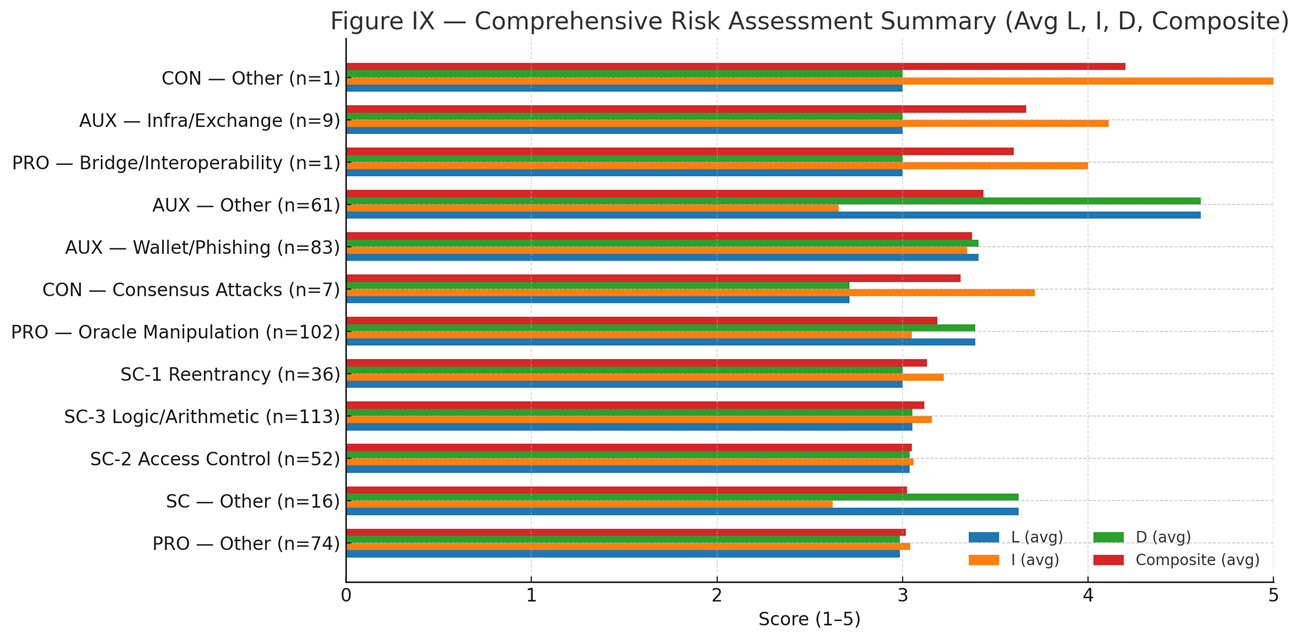
\includegraphics[width=0.4\textwidth]{../figure/Fig11.png}
\caption{Comprehensive risk assessment summary showing average likelihood (L), impact (I), detectability (D), and composite risk scores across all analyzed categories. Smart contract reentrancy attacks show the highest overall risk, while consensus layer attacks have the highest potential impact despite lower frequency.}
\label{fig:risk_scores_summary}
\end{figure}
